\chapter{Ensayos y resultados} % Main chapter title

\label{Chapter4}

Este capítulo presenta los ensayos realizados para validar la funcionalidad de
los componentes del sistema, tanto de manera individual como en conjunto. Se
presentan los resultados obtenidos y su análisis.

\section{Banco de pruebas}

Se construyó un banco de prueba físico con el objetivo de validar el
rendimiento, la funcionalidad y la integración de los sensores, actuadores y
módulos del sistema. Este entorno controlado permitió montar los dispositivos,
realizar el conexionado correspondiente y simular condiciones cercanas a las
reales de operación, lo que permitió evaluar el comportamiento general del
sistema. El banco de prueba incluyó los siguientes componentes:

\begin{itemize}
    \item \textbf{Sensores y actuadores:}
          \begin{itemize}
              \item Nodo ambiental: incluye los sensores BMP280, BH1750 y MH-Z19C.
              \item Nodo de consumos: compuesto por un módulo PZEM-004T y seis sensores HC-SR04.
              \item Nodo de solución nutritiva: equipado con un sensor de temperatura DS18B20,
                    sensores de pH, CE, TDS y un sensor HC-SR04.
              \item Nodo actuador: integrado por un módulo de relés de 4 canales (5 V, 10 A) y tres
                    módulos de relés de 2 canales (5 V, 10 A).
          \end{itemize}

    \item \textbf{Microcontroladores:}
          \begin{itemize}
              \item Cuatro módulos ESP-WROOM-32, uno por cada nodo.
              \item Cuatro placas base \cite{PlacaBaseESP32} para los módulos ESP-WROOM-32 para
                    facilitar la conexión de los módulos a los sensores y actuadores.
          \end{itemize}

    \item \textbf{Fuentes de alimentación:}
          \begin{itemize}
              \item Una fuente de 5 V, 2 A para los relés.
              \item Cuatro fuentes de 5 V, 1.5 A para los microcontroladores.
          \end{itemize}

    \item \textbf{Servidor MQTT:}
          \begin{itemize}
              \item El servicio se implementó en AWS IoT Core.
          \end{itemize}

    \item \textbf{Servidor web:}
          \begin{itemize}
              \item El backend, frontend y la base de datos se desplegaron en una máquina virtual
                    EC2 de AWS, a través del entorno de laboratorio provisto por \textit{AWS
                        Academy Learner Lab}.
          \end{itemize}
\end{itemize}

La figura \ref{fig:banco_pruebas} muestra el banco de pruebas utilizado para la
validación del sistema, donde se observan los sensores, actuadores,
microcontroladores y la alimentación eléctrica.

\begin{figure}[H]
    \centering
    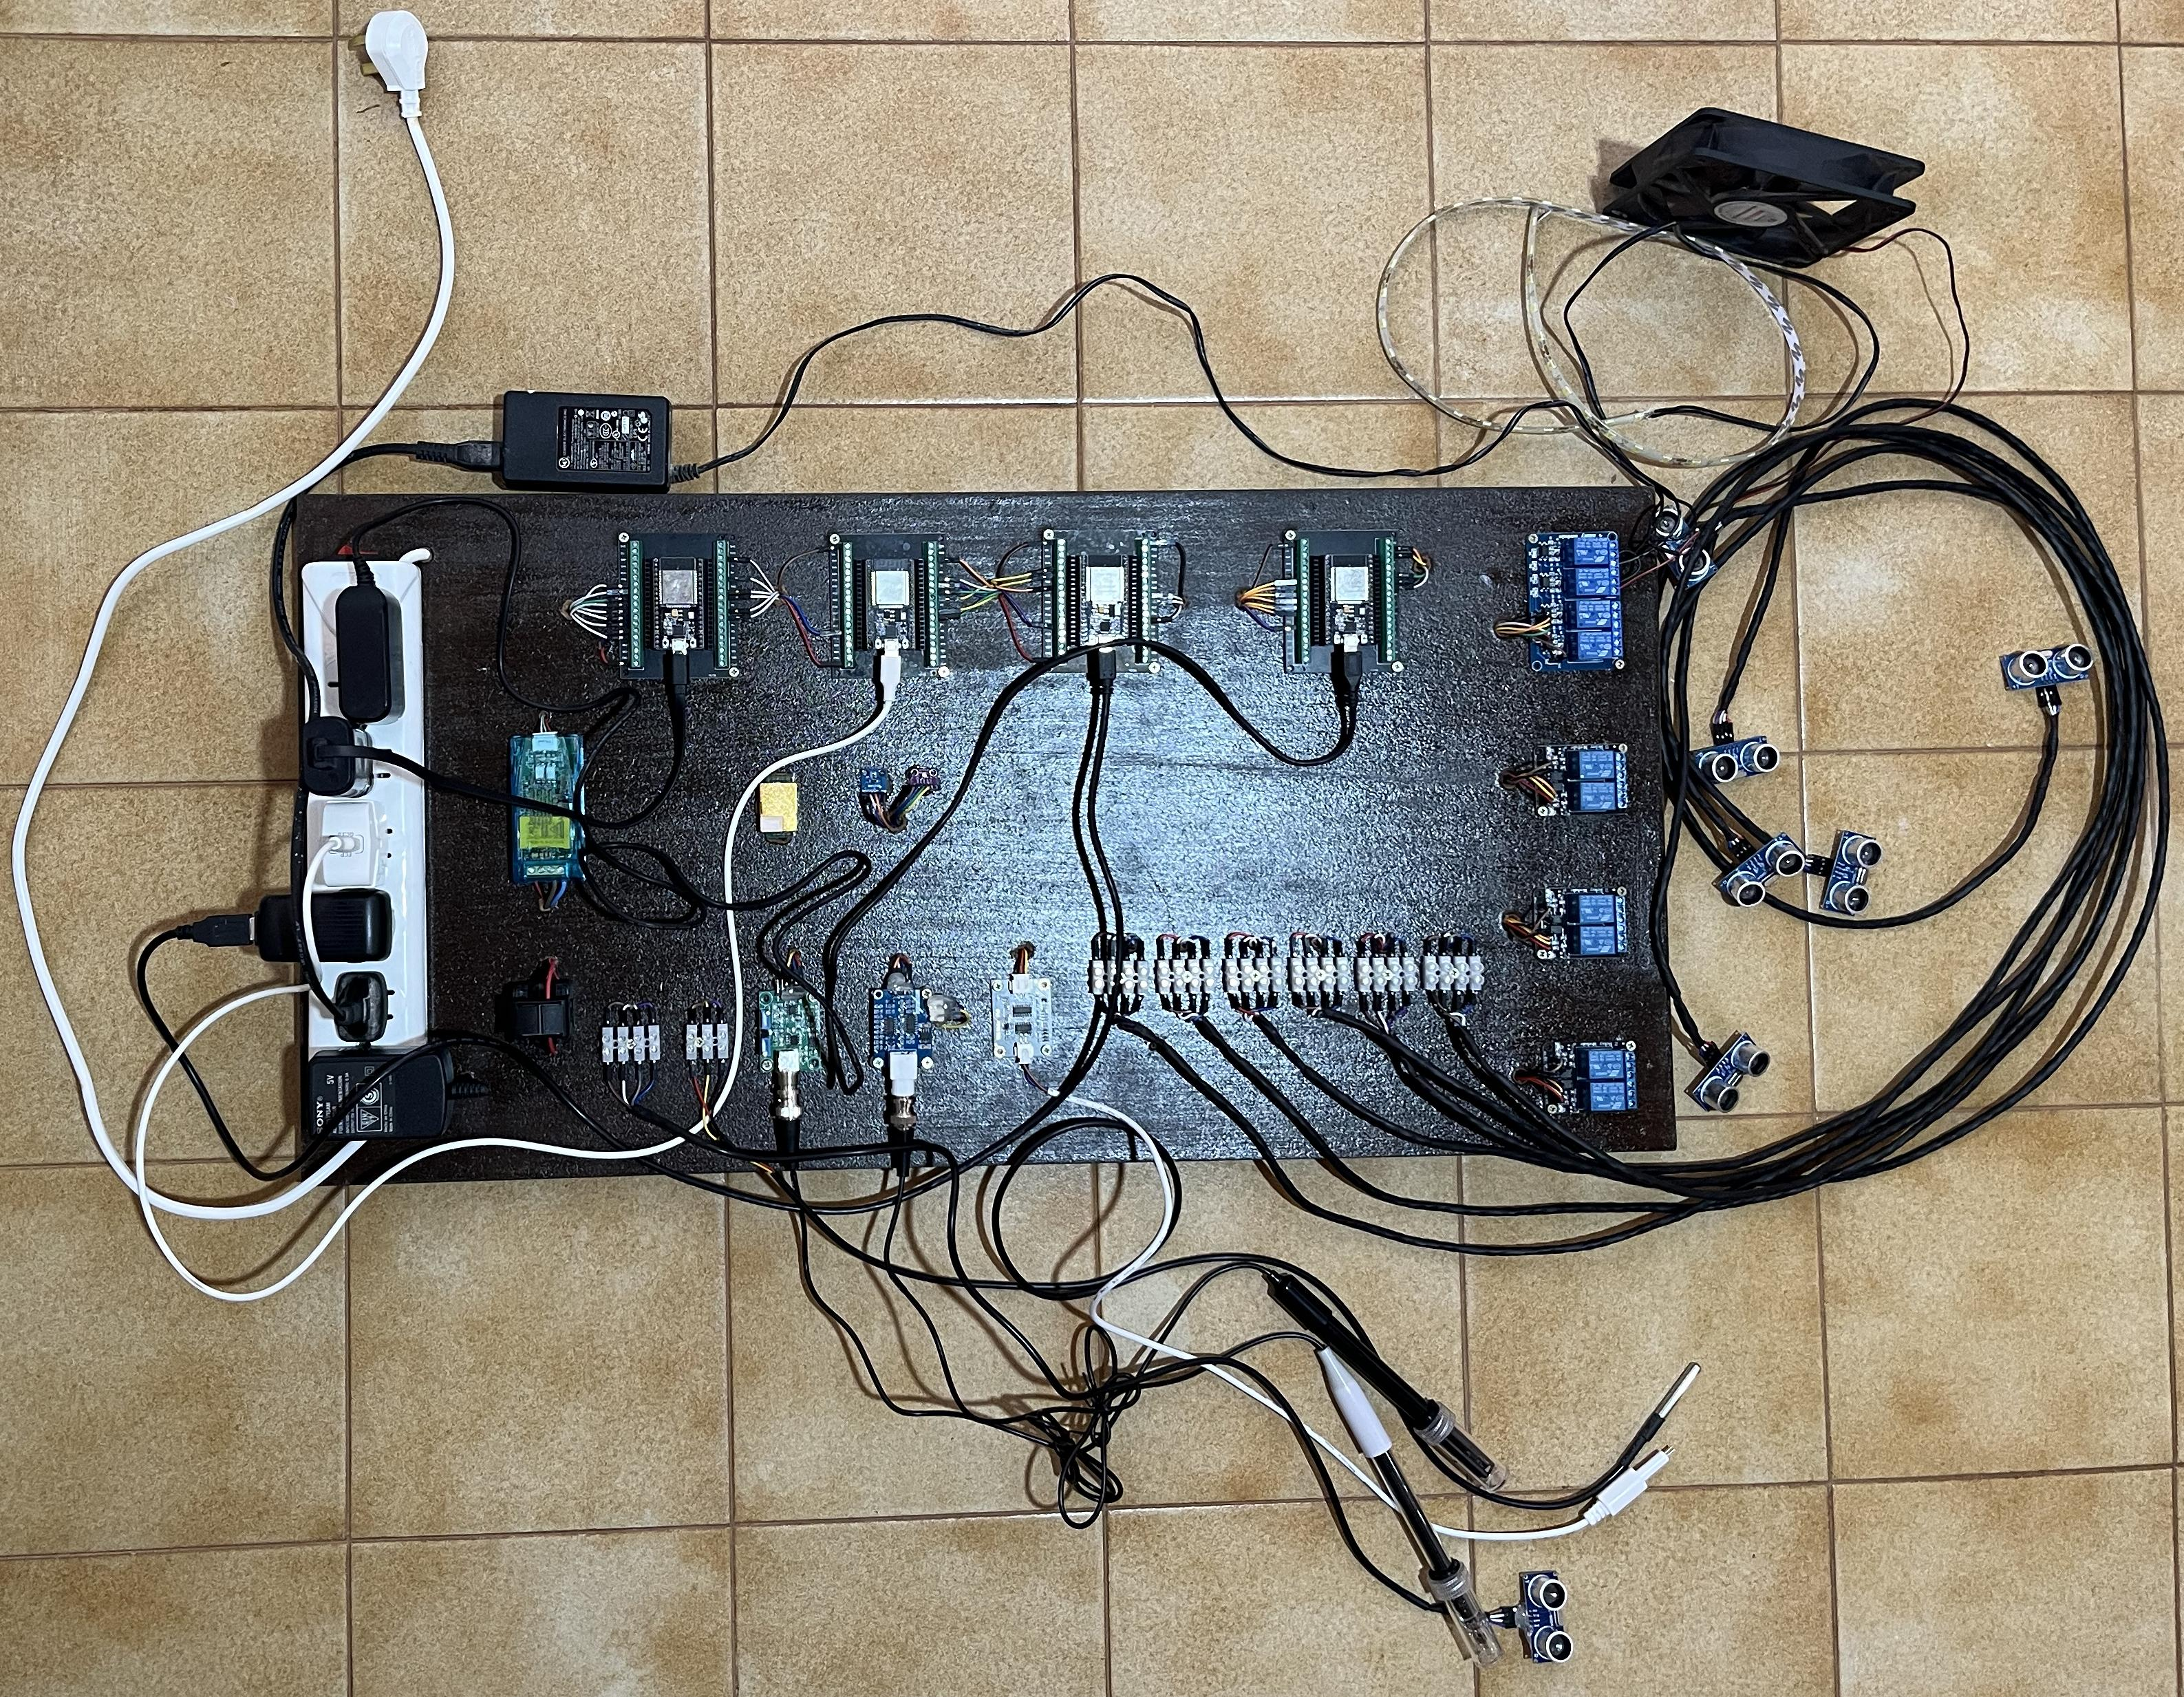
\includegraphics[width=0.95\textwidth]{Images/36_prototipo.jpeg}
    \caption[Banco de pruebas del sistema EnviroSenseIoT]{Banco de pruebas del sistema \texttt{EnviroSenseIoT}.}
    \label{fig:banco_pruebas}
\end{figure}

\section{Criterios de evaluación}

Una vez construido el banco de pruebas, se definieron criterios específicos
para evaluar el desempeño del sistema en términos de funcionalidad,
comunicación e integración. Las pruebas se enfocaron en verificar el correcto
funcionamiento de cada componente de forma individual (sensores, actuadores,
backend y frontend) y también en su comportamiento integrado como sistema
completo.

Se realizaron ensayos para comprobar la lectura de los sensores, la activación
de actuadores, la comunicación entre microcontroladores y el servidor web
mediante el protocolo MQTT, así como la correcta gestión de datos en el backend
y la usabilidad de la interfaz web. Estas validaciones permitieron identificar
el cumplimiento de los objetivos funcionales establecidos para cada módulo.

La tabla \ref{tab:criterios_evaluacion} resume los criterios aplicados durante
el proceso de validación en el entorno de prueba.

\begin{table}[H]
    \centering
    \caption[Criterios de evaluación del banco de pruebas]{Criterios de evaluación del banco de pruebas.}
    \begin{tabular}{p{3.4cm}p{3cm}p{6cm}}
        \hline
        \textbf{Criterio}                          & \textbf{Componente} & \textbf{Descripción}                                                                                                         \\
        \hline
        Verificación de endpoints y almacenamiento & Backend             & Comprobación del funcionamiento de los endpoints y del registro de información en la base de datos.                          \\
        \hline
        Usabilidad de la interfaz web              & Frontend            & Evaluación de la facilidad de uso y el acceso a funcionalidades.                                                             \\
        \hline
        Verificación de mediciones                 & Microcontroladores  & Verificación de los valores reportados por los sensores.                                                                     \\
        \hline
        Activación de actuadores                   & Microcontroladores  & Validación de la activación de los módulos de relés ante eventos enviados.                                                   \\
        \hline
        Verificación de comunicación MQTT          & Comunicación MQTT   & Verificación de la comunicación entre microcontroladores y servidor web a través del intercambio de mensajes en los tópicos. \\
        \hline
        Integración de módulos                     & Todo el sistema     & Verificación del funcionamiento conjunto de sensores, actuadores y servidor web.                                             \\
        \hline
    \end{tabular}
    \label{tab:criterios_evaluacion}
\end{table}

\section{Pruebas de backend}
\label{sec:pruebas_backend}

El backend del sistema cuenta con un total de 111 endpoints, a través de los
cuales se realiza la interacción con los distintos módulos y servicios. Para su
validación, se utilizó la herramienta Postman, que permitió realizar pruebas
funcionales destinadas a verificar que cada endpoint respondiera correctamente
a las solicitudes y devolviera los datos esperados conforme a la lógica
definida.

% Adicionalmente, el sistema incluye una interfaz Swagger \cite{SwaggerIO}, que
% facilita tanto la documentación como la validación interactiva de los
% endpoints. Esta interfaz permite explorar las operaciones disponibles,
% visualizar los parámetros requeridos y ejecutar pruebas directamente desde el
% navegador, sin necesidad de recurrir a herramientas externas.

% La Figura \ref{fig:swagger} ilustra la interfaz de Swagger, donde se presentan
% los distintos endpoints organizados por categoría. Cada uno puede expandirse
% para consultar detalles de las solicitudes y respuestas, acceder a ejemplos y
% evaluar su comportamiento en tiempo real.

Además, FastAPI incorpora una interfaz Swagger \cite{SwaggerIO}, que permite
documentar, explorar y probar los endpoints desde el navegador. La Figura
\ref{fig:swagger} muestra esta interfaz, donde los endpoints se organizan por
categoría y pueden consultarse y evaluarse en tiempo real.

\begin{figure}[H]
    \centering
    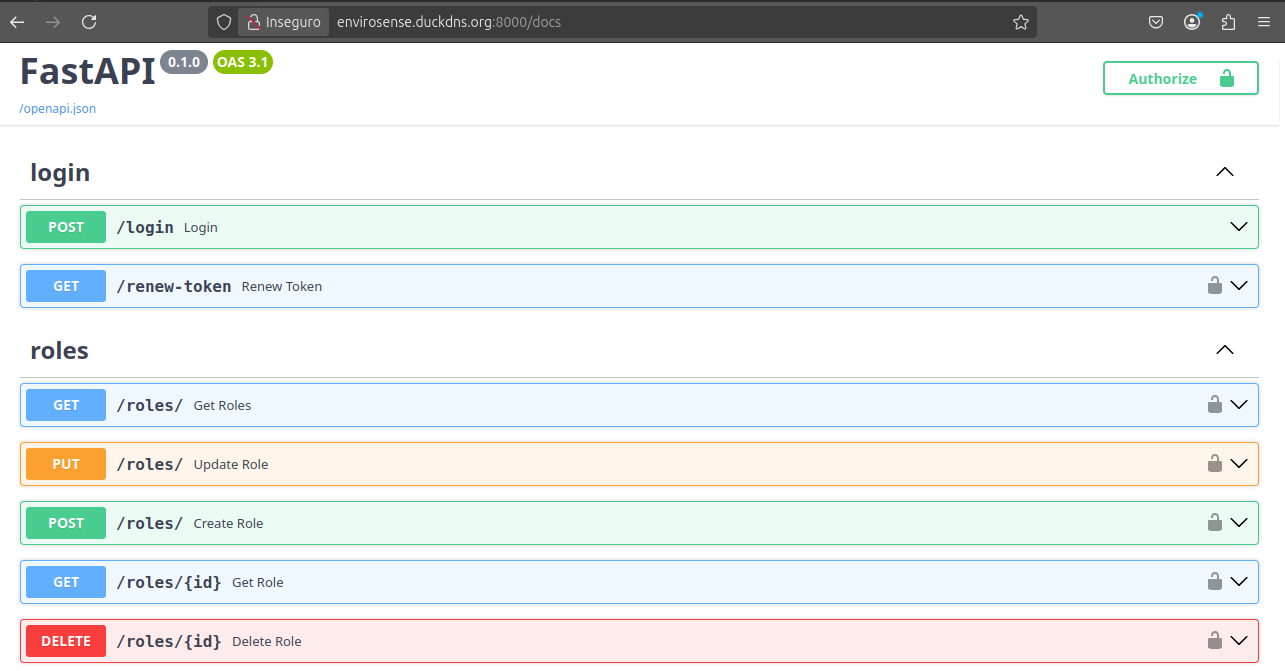
\includegraphics[width=\textwidth]{Images/37_swagger.png}
    \caption[Interfaz de Swagger]{Interfaz de Swagger.}
    \label{fig:swagger}
\end{figure}

\subsection{Pruebas en Postman}

En el repositorio de GitHub \cite{EnviroSenseIoT} se encuentra la carpeta
\texttt{Tests}, que contiene un archivo JSON con la colección completa de
pruebas realizadas con Postman. Dicha colección abarca todos los endpoints del
backend evaluados, junto con los resultados correspondientes.

Tambien se incluyen un archivo CSV (del inglés \textit{Comma Separated Values})
y un archivo en formato texto, en el que se detallan los endpoints, los métodos
HTTP, los resultados obtenidos y el promedio, para permitir una trazabilidad
clara del proceso de validación.

La figura \ref{fig:postman} presenta un ejemplo de las pruebas realizadas en
Postman, donde se detalla la respuesta de los endpoints, el método HTTP
utilizado, la URL del endpoint, el código de estado, el tiempo y el tamaño de
la respuesta.

\begin{figure}[H]
    \centering
    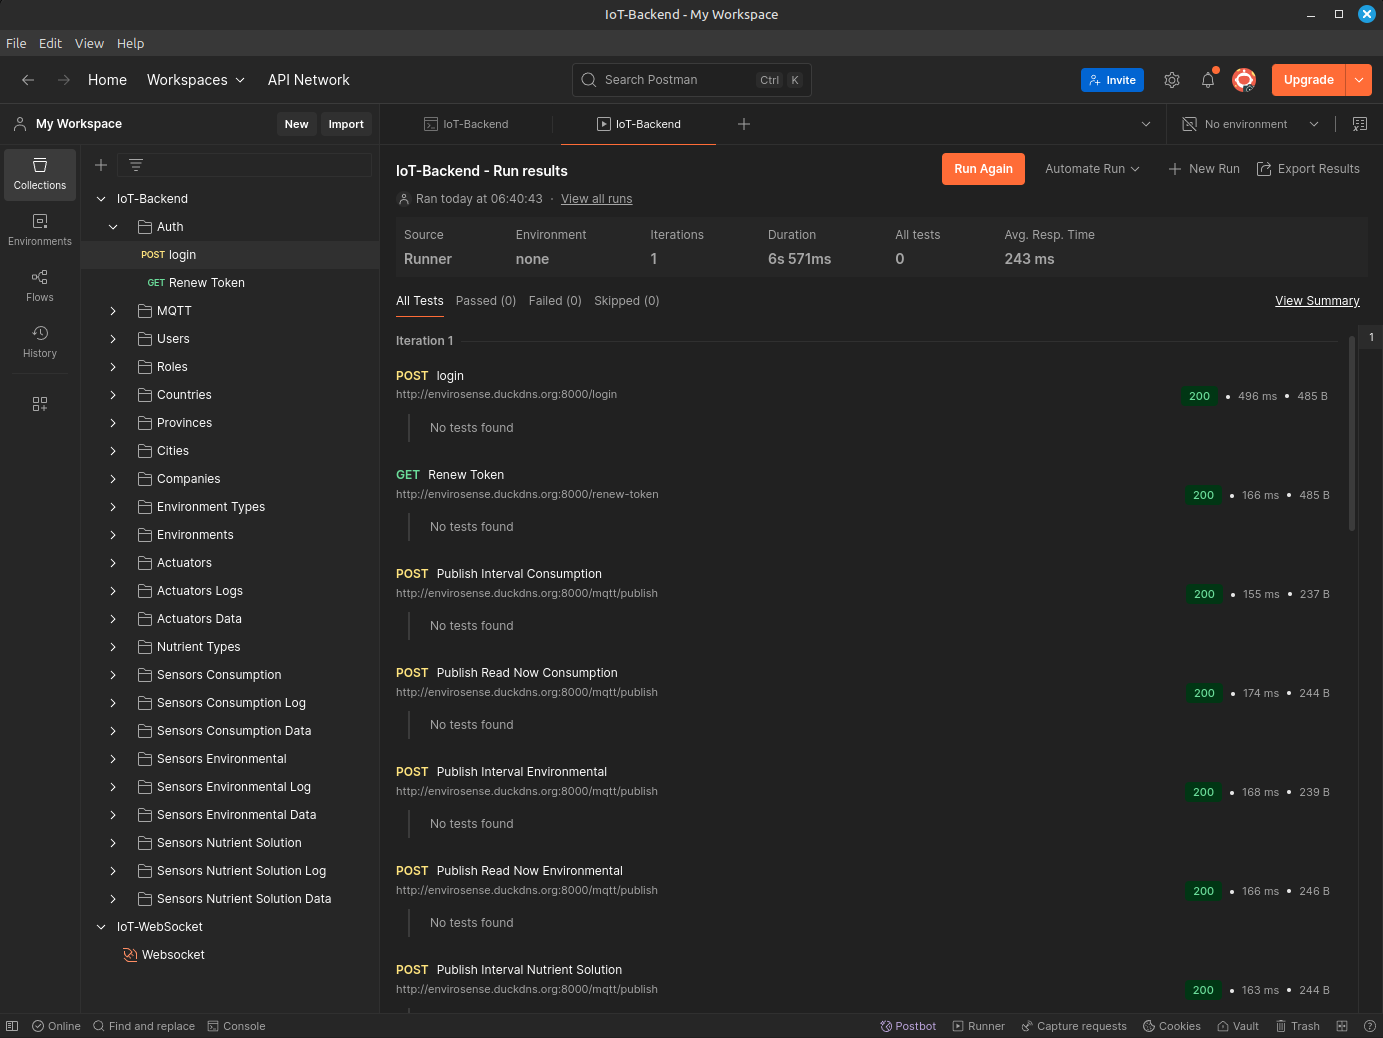
\includegraphics[width=\textwidth]{Images/38_postman.png}
    \caption[Pruebas realizadas en Postman]{Pruebas realizadas en Postman.}
    \label{fig:postman}
\end{figure}

\subsubsection{Evaluación general}

Los tiempos de respuesta obtenidos durante las pruebas fueron, en su mayoría,
adecuados para un entorno compuesto por servicios desplegados en contenedores
Docker dentro de una instancia EC2 de AWS. El promedio se mantuvo cercano a los
200 ms, valor que garantiza una experiencia de usuario satisfactoria y un
rendimiento eficiente del sistema.

Las operaciones más exigentes, como las consultas filtradas sobre grandes
volúmenes de datos o el cambio de contraseñas, presentaron tiempos de respuesta
ligeramente superiores. Sin embargo, se mantuvieron dentro de márgenes
aceptables, al considerar la complejidad de estas tareas y las características
del entorno de ejecución en la nube.

La Tabla \ref{tab:tiempos_respuesta} presenta los resultados obtenidos durante
las pruebas de desempeño, organizados por categoría funcional. Se detallan los
métodos evaluados y los tiempos de respuesta registrados, lo que permite
analizar el comportamiento del sistema ante distintos tipos de solicitudes.

\begin{table}[H]
    \centering
    \caption[Resultados de tiempos de respuesta]{Resultados de tiempos de respuesta de las pruebas.}
    \begin{tabular}{p{5cm}p{5.1cm}p{2.4cm}}
        \toprule
        \textbf{Categoría}                                                     & \textbf{Método}                             & \textbf{Tiempo de Respuesta} \\
        \midrule
        \multirow{3}{5cm}{Autenticación y usuarios}                            & POST Login                                  & 496 ms                       \\
                                                                               & GET Current User                            & 181 ms                       \\
                                                                               & PATCH Update Password                       & 827 ms                       \\
        \hline
        \multirow{3}{5cm}{Publicación de mensajes en MQTT y logs}              & POST Publish MQTT                           & 153 – 181 ms                 \\
                                                                               & GET Logs (actuadores y sensores)            & 173 – 193 ms                 \\
        \hline
        \multirow{2}{5cm}{Consulta de datos de dispositivos}                   & GET Sensors Data                            & $\sim$208 ms                 \\
                                                                               & GET Actuators Data                          & 271 ms                       \\
        \hline
        \multirow{3}{5cm}{Operaciones de creación, modificación y eliminación} & POST Create User / Company                  & $\sim$490 ms                 \\
                                                                               & POST Create Sensor / Data                   & 154 – 194 ms                 \\
                                                                               & PUT / DELETE                                & 161 – 188 ms                 \\
        \hline
        \multirow{4}{5cm}{Datos geográficos y configuración}                   & GET Countries / Provinces / Cities          & 176 – 187 ms                 \\
                                                                               & POST Create Environment / Actuator / Sensor & 179 – 194 ms                 \\
        \bottomrule
    \end{tabular}
    \label{tab:tiempos_respuesta}
\end{table}

El análisis de los tiempos de respuesta arrojó un promedio general de
\textbf{204.38 ms} sobre un total de \textbf{111 solicitudes}. Esta métrica
refuerza la conclusión de que el sistema opera de manera eficiente dentro del
entorno en la nube.

La tabla \ref{tab:promedios_metodo_http} presenta la distribución de los
tiempos de respuesta por método HTTP. Además, se observó un comportamiento
diferenciado según el tipo de operación solicitada, como se resume a
continuación:

\begin{table}[H]
    \centering
    \caption[Promedios de tiempos de respuesta]{Promedios de tiempos de respuesta por método HTTP.}
    \begin{tabular}{ l l }
        \toprule
        \textbf{Método HTTP} & \textbf{Tiempo de Respuesta} \\
        \midrule
        GET                  & 191.0 ms (46 solicitudes)    \\
        POST                 & 199.47 ms (36 solicitudes)   \\
        PUT                  & 202.64 ms (14 solicitudes)   \\
        DELETE               & 195.77 ms (13 solicitudes)   \\
        PATCH                & 668.5 ms (2 solicitudes)     \\
        \bottomrule
    \end{tabular}
    \label{tab:promedios_metodo_http}
\end{table}

\subsubsection{Resultados generales de las pruebas}

A continuación, se resumen los principales resultados obtenidos durante las
pruebas realizadas en Postman:

\begin{itemize}
    \item Todas las pruebas fueron exitosas, sin registrar errores en el backend ni
          fallos en las respuestas.
    \item Los tiempos de respuesta se mantuvieron estables y apropiados para un sistema
          desplegado en contenedores sobre infraestructura en la nube.
    \item Las operaciones clave, como la autenticación, la creación de entidades y las
          consultas de datos, mostraron tiempos de respuesta ligeramente superiores, pero
          no afectaron la experiencia del usuario. El rendimiento se mantuvo
          satisfactorio en el entorno de prueba con servicios en la nube.
\end{itemize}

\subsection{Pruebas de validación de WebSocket}

% Para validar el funcionamiento de la comunicación en tiempo real mediante
% WebSocket, se realizaron pruebas orientadas a verificar la conexión persistente
% entre múltiples clientes simultáneos y el servidor backend, así como el
% correcto envío y recepción de mensajes. Se utilizaron como clientes tanto
% Postman como navegadores web, lo que permitió establecer conexiones WebSocket
% entre el frontend y el backend.

% Se comprobó la estabilidad de la conexión, la capacidad del backend para enviar
% mensajes a los clientes conectados y la recepción inmediata de los datos por
% parte de estos. Los resultados obtenidos confirmaron la eficiencia y
% confiabilidad del canal WebSocket implementado.

% La figura \ref{fig:websocket} muestra un ejemplo de la conexión WebSocket entre
% el frontend y el backend. A la izquierda, se observa la conexión establecida
% desde el frontend; a la derecha, las realizadas mediante Postman. También se
% visualiza una terminal de Linux conectada al backend en una instancia de AWS
% EC2, donde se evidencia la conexión activa de tres clientes simultáneos.

Para validar la comunicación en tiempo real mediante WebSocket, se ejecutaron
pruebas que verificaron la conexión persistente entre múltiples clientes
simultáneos y el servidor backen y el envío y la recepción de mensajes.

Los clientes incluyeron instancias en Postman y navegadores web, lo que
permitió establecer conexiones WebSocket entre el frontend y el backend.

Las pruebas confirmaron la estabilidad en las conexiones, la capacidad del
backend para distribuir mensajes a todos los clientes conectados y la recepción
inmediata de datos en los clientes.

Los resultados demostraron la eficiencia y confiabilidad del canal WebSocket
implementado. La figura \ref{fig:websocket} ilustra un ejemplo de la conexión
WebSocket entre el frontend y el backend. A la izquierda, se observa la
conexión establecida desde el frontend; a la derecha, las realizadas mediante
Postman. También se visualiza una terminal de Linux conectada al backend en una
instancia de AWS EC2, donde se evidencia la conexión activa de tres clientes
simultáneos.

\begin{figure}[H]
    \centering
    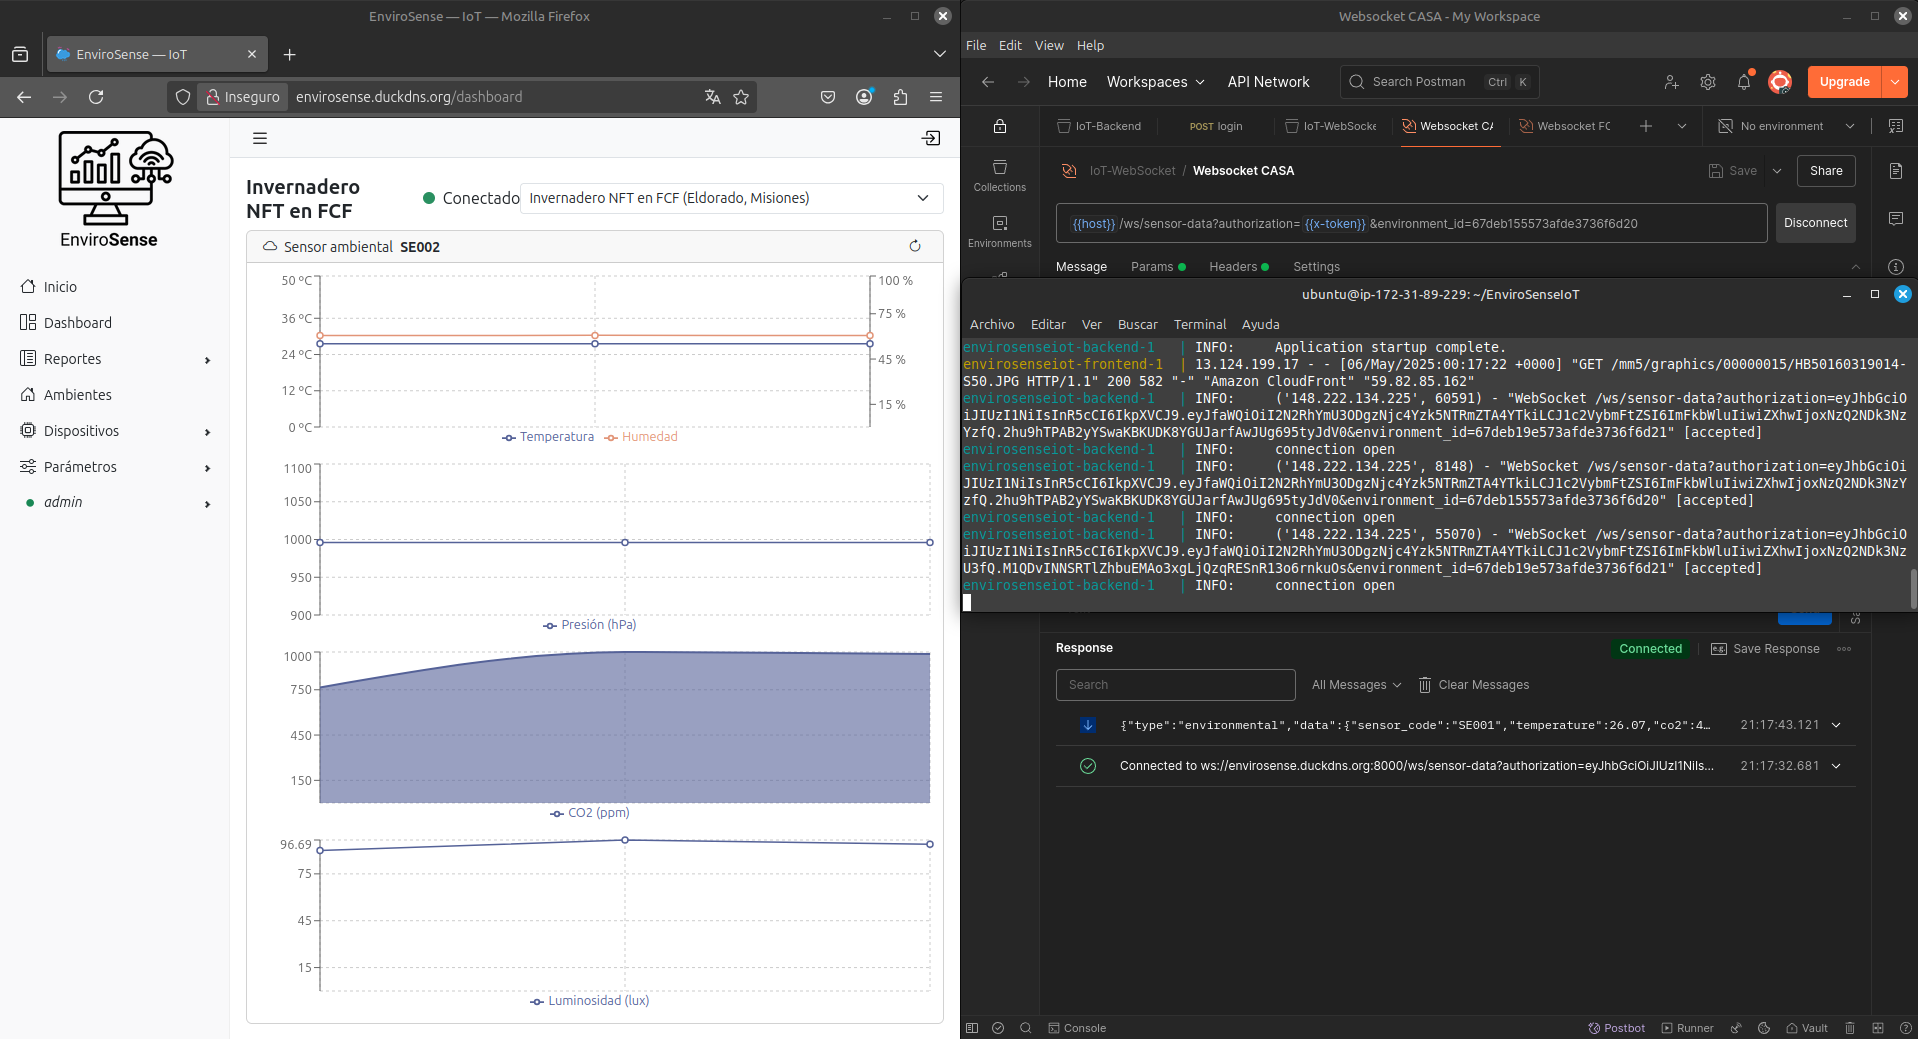
\includegraphics[width=\textwidth]{Images/40_websocket.png}
    \caption[Pruebas de WebSocket]{Pruebas de WebSocket.}
    \label{fig:websocket}
\end{figure}

\subsection{Pruebas de validación de almacenamiento en MongoDB}

Se llevaron a cabo pruebas para validar el almacenamiento de los datos en
MongoDB, con el objetivo de comprobar que las operaciones de escritura
realizadas desde el backend, tales como la creación de usuarios, sensores,
mediciones y eventos, se registraran en las colecciones correspondientes.

Para ello, se realizaron las siguientes acciones:

\begin{itemize}
    \item Se ejecutaron operaciones desde Postman, para generar nuevas entidades en el
          sistema.
    \item A continuación, se accedió directamente a la base de datos MongoDB, a través de
          la herramienta MongoDB Compass \cite{MongoDBCompass}, para inspeccionar las
          colecciones y verificar la existencia y la estructura de los documentos
          insertados.
    \item Se validó que las operaciones de actualización y eliminación impactaran
          correctamente sobre los documentos correspondientes en MongoDB.
\end{itemize}

Estas validaciones permitieron confirmar que el backend realiza una correcta
persistencia de los datos en MongoDB y que no se observaron inconsistencias, ni
pérdidas de información durante las operaciones.

La figura \ref{fig:mongodb} ilustra un ejemplo del proceso de creación de un
nuevo usuario. Se muestra la solicitud enviada desde Postman junto con la
respuesta proporcionada por el servidor. Asimismo, en la interfaz de MongoDB
Compass se visualiza el nuevo usuario incorporado en la colección \texttt{User}
de la base de datos.

\begin{figure}[H]
    \centering
    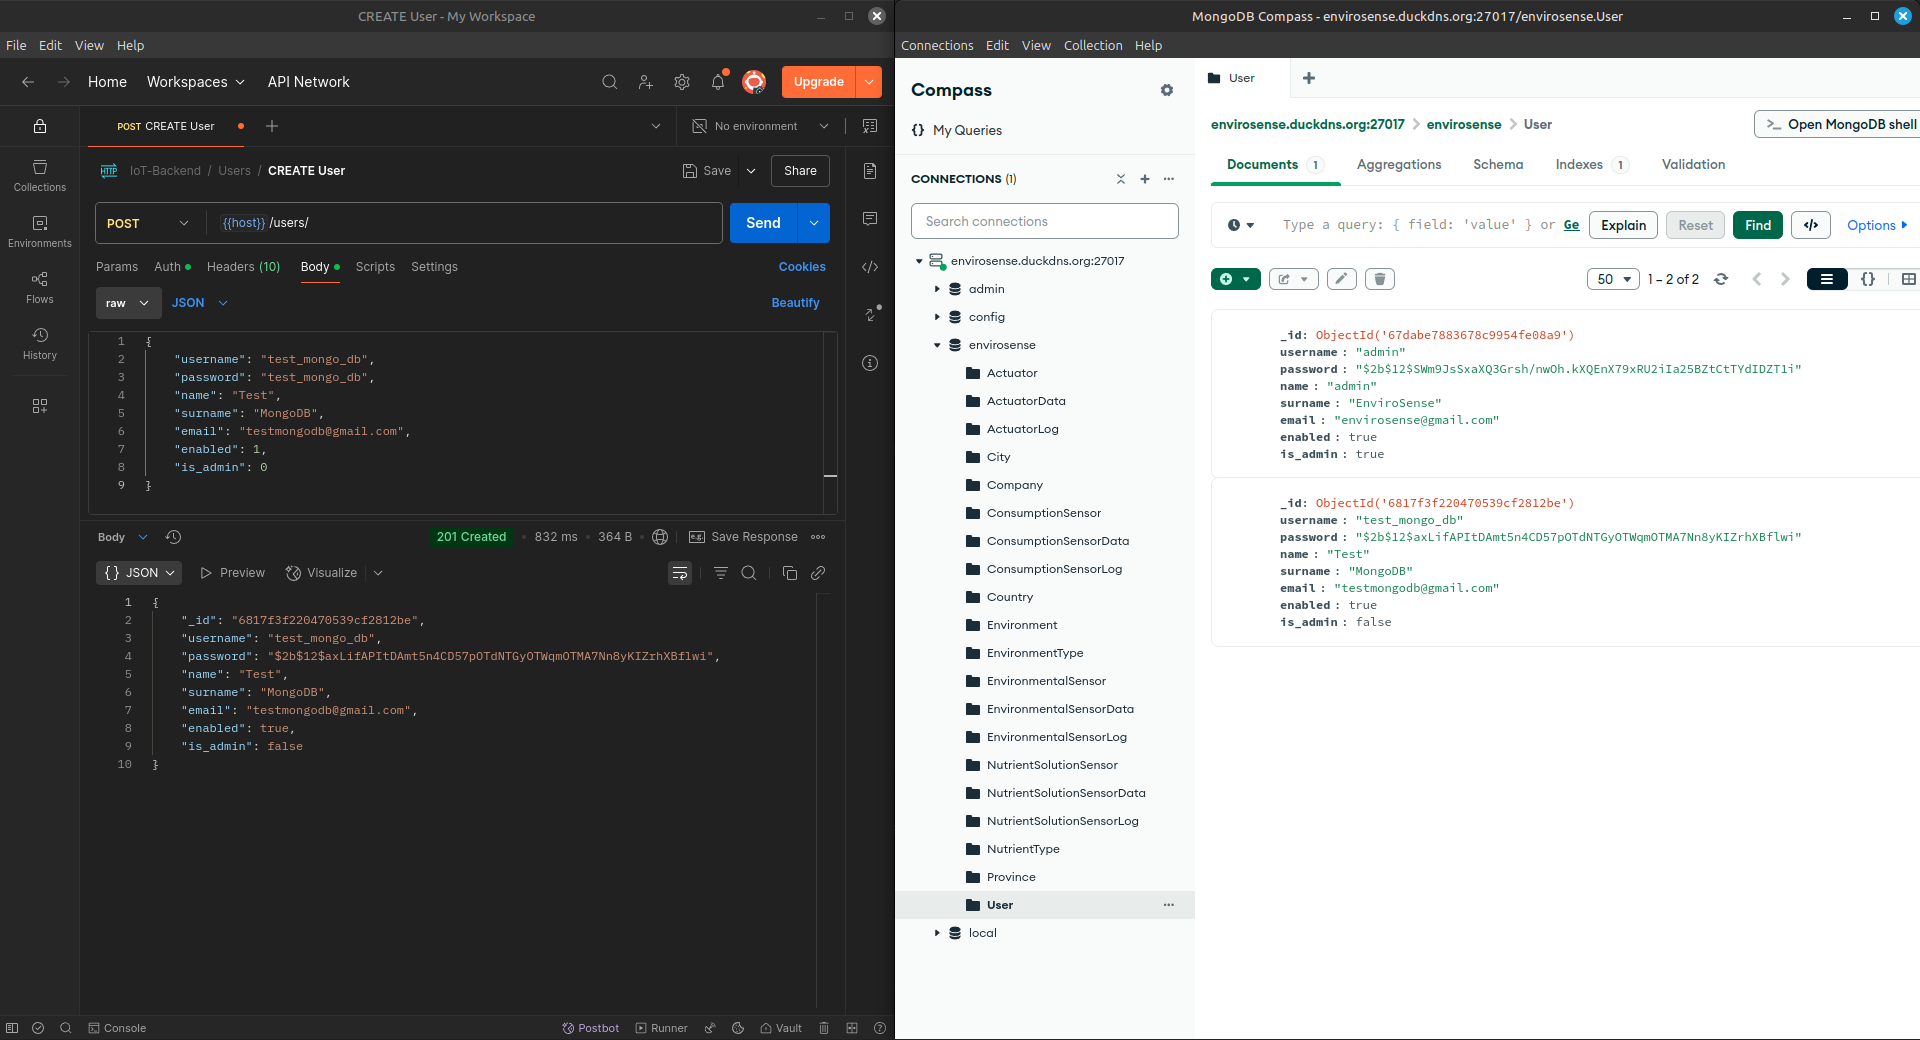
\includegraphics[width=\textwidth]{Images/39_test_mongodb.png}
    \caption[Validación de almacenamiento en MongoDB]{Validación de almacenamiento en MongoDB.}
    \label{fig:mongodb}
\end{figure}

% \subsection{conclusión de pruebas realizadas al backend}

% Las pruebas efectuadas sobre el backend confirmaron el correcto funcionamiento
% y la capacidad para responder adecuadamente a las distintas solicitudes. Los
% tiempos de respuesta permiten asegurar una experiencia de usuario
% satisfactoria, y se verificó con éxito la persistencia de los datos en MongoDB.

% Además, se validó la comunicación en tiempo real mediante WebSocket y se
% comprobó la estabilidad de la conexión persistente entre múltiples clientes
% simultáneos y el backend. Las pruebas demostraron que la API transmite datos de
% manera inmediata a todos los clientes conectados, lo que destaca la eficiencia
% y confiabilidad del canal WebSocket implementado.

% El backend demostró una operabilidad sólida, permitió la gestión y
% actualización continua de datos de manera confiable y garantizó la integridad y
% la persistencia de la información a lo largo del tiempo.

\section{Pruebas de frontend}
\label{sec:pruebas_frontend}

Las pruebas realizadas al frontend se centraron en evaluar la seguridad, la
usabilidad y la funcionalidad de la interfaz web. Se llevaron a cabo pruebas de
autenticación, autorización y acceso a los distintos módulos del sistema. Se
validó la correcta visualización de los datos, la interacción con los
componentes y la capacidad de respuesta ante diferentes acciones del usuario.

Las validaciones incluyeron:

\begin{itemize}
    \item Pruebas de autenticación y autorización: se verificó que los usuarios pudieran
          iniciar sesión correctamente y acceder a las funcionalidades correspondientes a
          su rol.
    \item Pruebas de funcionalidad: se validó que todas las funcionalidades implementadas
          en el frontend funcionaran correctamente.
    \item Pruebas de usabilidad: se evaluó la facilidad de uso de la interfaz y su
          responsividad, para garantizar que los usuarios pudieran navegar sin
          dificultades, realizar las acciones deseadas y acceder de manera óptima desde
          diferentes dispositivos y tamaños de pantalla.
\end{itemize}

\subsection{Pruebas de autenticación y autorización}

Las pruebas de autenticación y autorización se llevaron a cabo para garantizar
que los usuarios pudieran iniciar sesión correctamente y acceder a las
funcionalidades correspondientes a su rol. Se realizaron pruebas con diferentes
tipos de usuarios, como administradores y usuarios estándar, para verificar que
cada uno tuviera acceso a las funcionalidades adecuadas y que no pudieran
acceder a las funciones restringidas a otros roles.

\subsubsection{Pruebas de autenticación}

La figura \ref{fig:login} muestra un ejemplo de la pantalla de inicio de
sesión, donde se ingresan las credenciales de usuario. Para este ejemplo se
ingresa un usuario \texttt{admin} y una contraseña incorrecta. Se puede
observar que el sistema devuelve un mensaje de error en el cual indica que las
credenciales son incorrectas.

\begin{figure}[H]
    \centering
    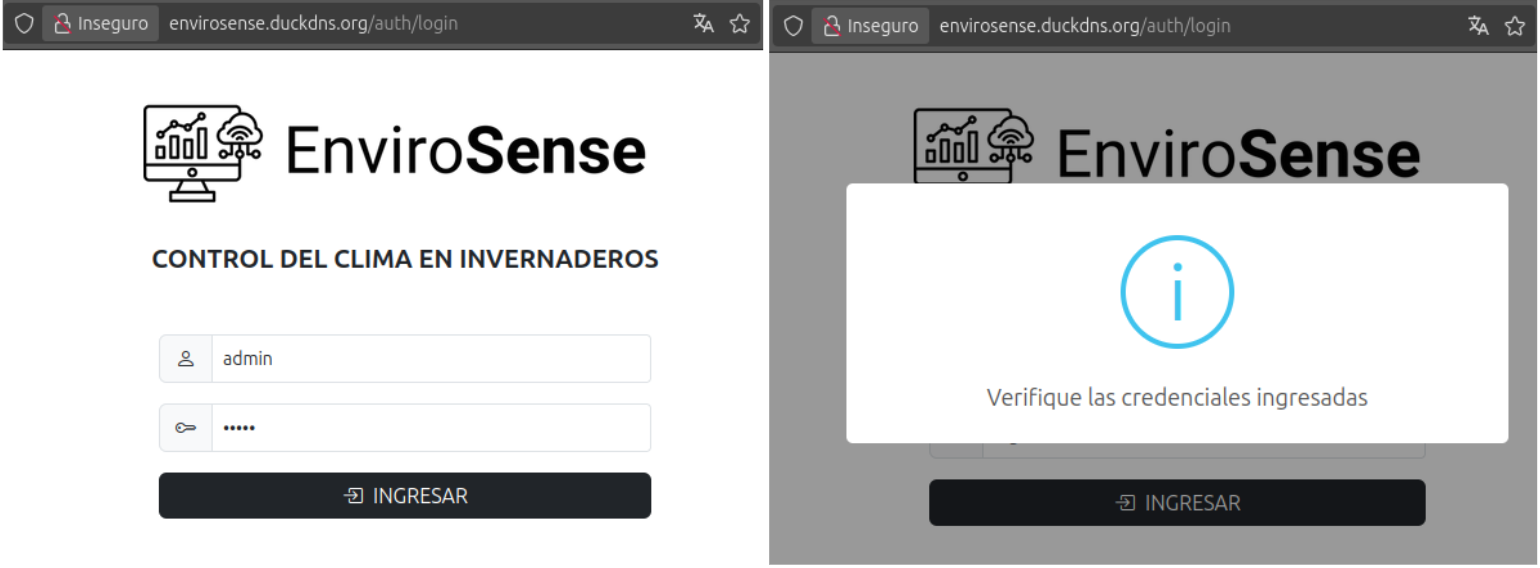
\includegraphics[width=\textwidth]{Images/41_intento_login.png}
    \caption[Pruebas de autenticación]{Pruebas de autenticación.}
    \label{fig:login}
\end{figure}

\subsubsection{Pruebas de autenticación y autorización}
Una vez que el usuario ingresa las credenciales correctas, se redirige a la
pantalla principal del sistema, donde se pueden observar las distintas
funcionalidades disponibles según el rol del usuario.

La figura \ref{fig:login_correcto_admin} ilustra el proceso de inicio de sesión
con un usuario \texttt{admin} y una contraseña válida. Al ingresar las
credenciales correctas, el sistema redirige al usuario a la pantalla principal,
donde se visualizan los módulos y funcionalidades disponibles, según el rol
asignado. En este caso, el usuario tiene acceso completo a todas las opciones
del sistema.

\begin{figure}[H]
    \centering
    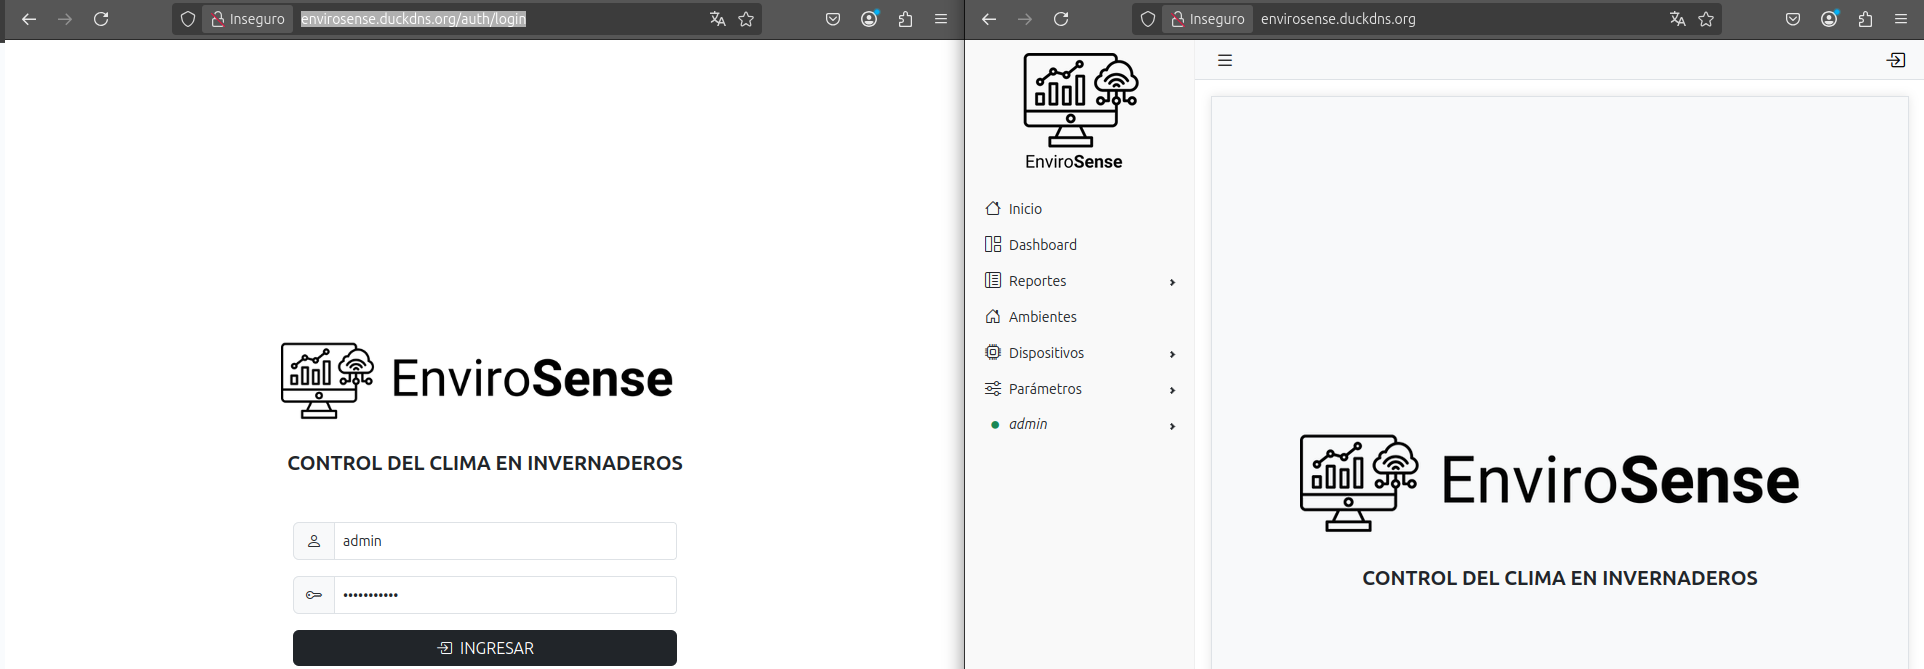
\includegraphics[width=\textwidth]{Images/42_login_correcto_admin.png}
    \caption[Autenticación y autorización rol administrador]{Autenticación y autorización de rol administrador.}
    \label{fig:login_correcto_admin}
\end{figure}

La figura \ref{fig:login_correcto_user} muestra el proceso de inicio de sesión
con un usuario estándar \texttt{martin} y una contraseña válida. Al ingresar
las credenciales correctas, el sistema redirige al usuario a la pantalla
principal, donde se pueden observar las distintas funcionalidades disponibles
según el rol del usuario. En este caso, el usuario tiene acceso limitado a las
opciones del sistema, lo que garantiza que solo pueda interactuar con las
funciones disponibles para su rol.

\begin{figure}[H]
    \centering
    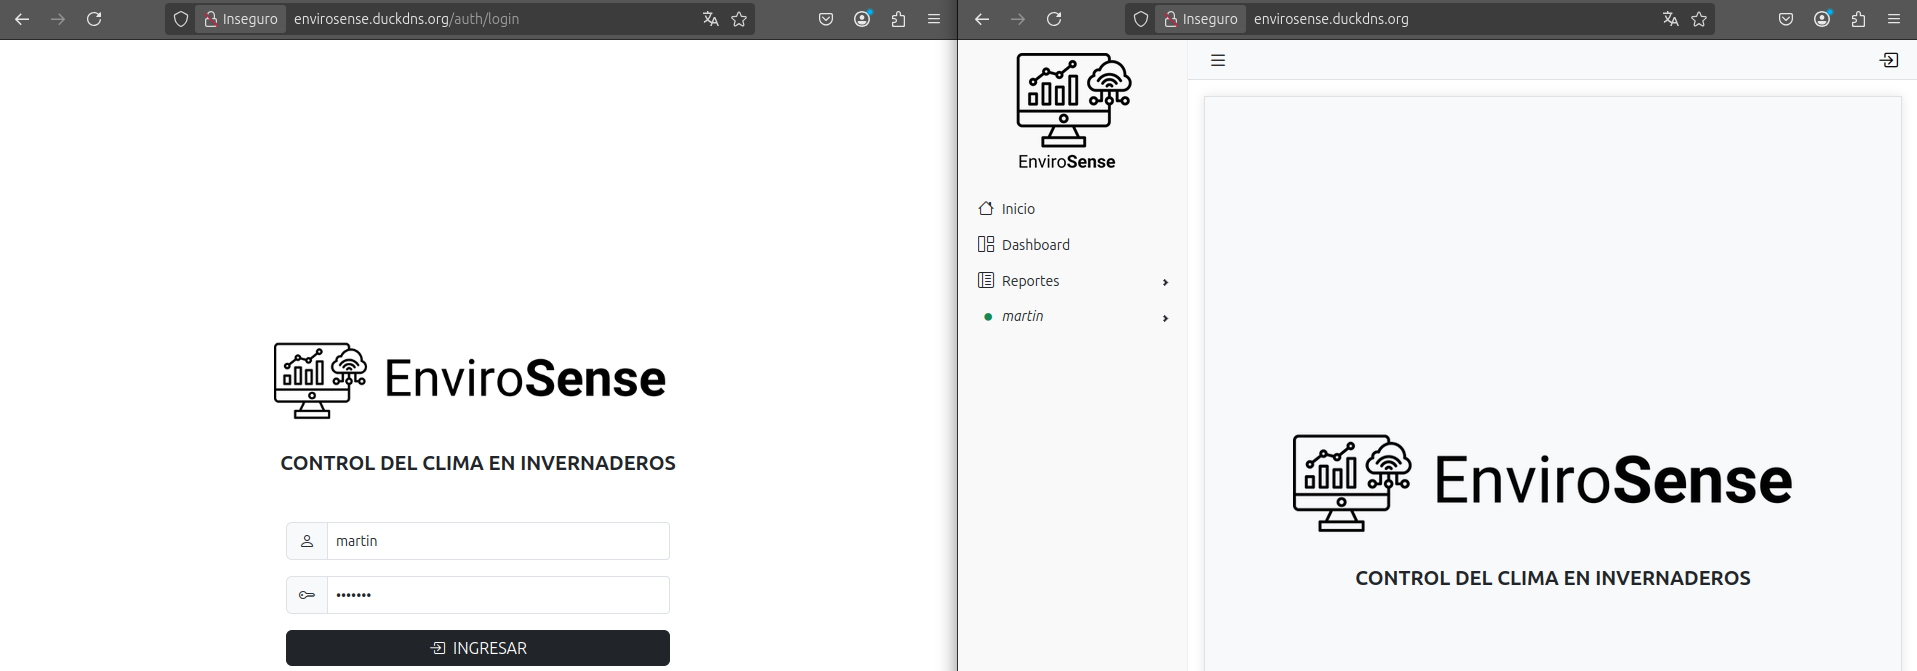
\includegraphics[width=\textwidth]{Images/43_login_correcto_user.png}
    \caption[Autenticación y autorización rol usuario]{Autenticación y autorización de rol usuario.}
    \label{fig:login_correcto_user}
\end{figure}

\subsection{Pruebas de funcionalidad}

Se realizaron pruebas exhaustivas para validar el correcto funcionamiento de
todas las funcionalidades del frontend. Se verificó que cada módulo respondiera
adecuadamente a las acciones del usuario y que los datos se visualizaran
correctamente en la interfaz.

\subsubsection{Validación de formularios}

Se verificó que los formularios cumplieran con las restricciones definidas,
como campos obligatorios, formatos específicos y límites de caracteres. También
se evaluó la correcta visualización de los mensajes de error ante entradas
inválidas.

La figura \ref{fig:formulario} muestra un ejemplo del formulario de creación de
usuario: en la imagen de la izquierda, el intento de envío con campos
incompletos activa mensajes de advertencia; en la imagen de la derecha, al
ingresar todos los datos requeridos, el sistema valida correctamente la
información y muestra un mensaje de confirmación previo a la creación del nuevo
usuario.

\begin{figure}[H]
    \centering
    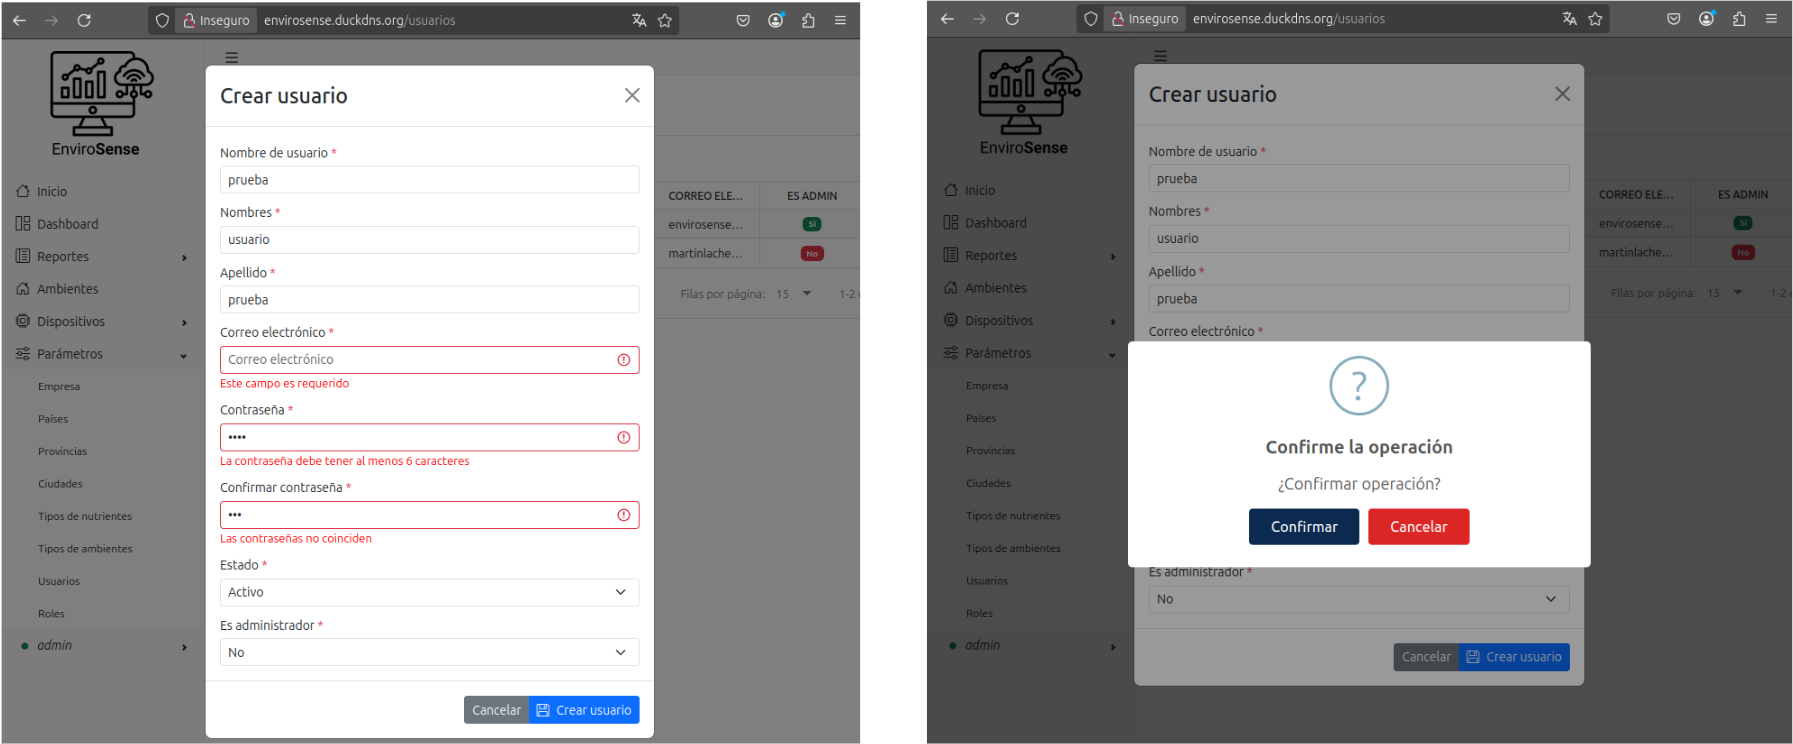
\includegraphics[width=\textwidth]{Images/44_formulario.png}
    \caption[Validación de formularios]{Validación de formularios.}
    \label{fig:formulario}
\end{figure}

La figura \ref{fig:verificacion_formulario} permite verificar la creación del
usuario \texttt{prueba} en la base de datos. El registro se visualiza en la
tabla de usuarios, donde se reflejan correctamente todos los datos ingresados
previamente en el formulario.

\begin{figure}[H]
    \centering
    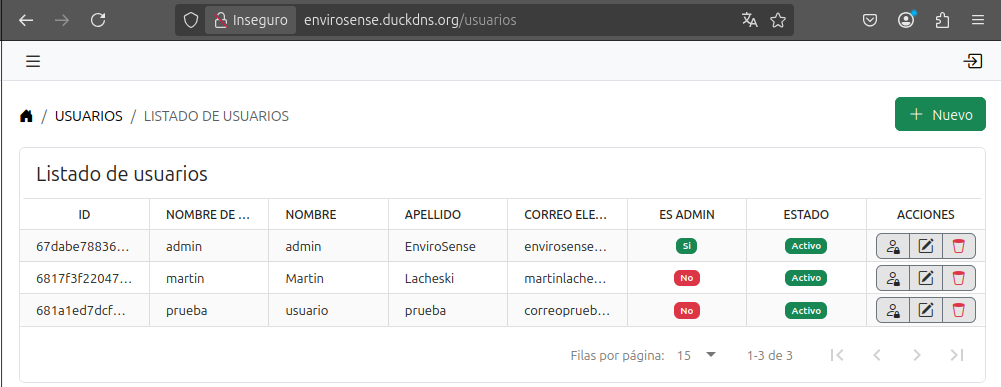
\includegraphics[width=\textwidth]{Images/44_formulario_verificacion.png}
    \caption[Verificación de creación de usuario]{Verificación de creación de usuario.}
    \label{fig:verificacion_formulario}
\end{figure}

\subsubsection{Validación de tablas y gráficos}

Se verificó la correcta visualización de las tablas, así como el funcionamiento
de la paginación y el filtrado. También se evaluaron los gráficos, se comprueba
su claridad, precisión y actualización dinámica frente a cambios en los datos.

La figura \ref{fig:tabla} presenta un ejemplo de los reportes del sensor
ambiental. En la parte superior se encuentra el formulario para seleccionar
sensor, rango de fechas y nivel de agregación; en el centro, la tabla con los
datos generados; y abajo, el sistema de paginación para navegar los registros.

\begin{figure}[H]
    \centering
    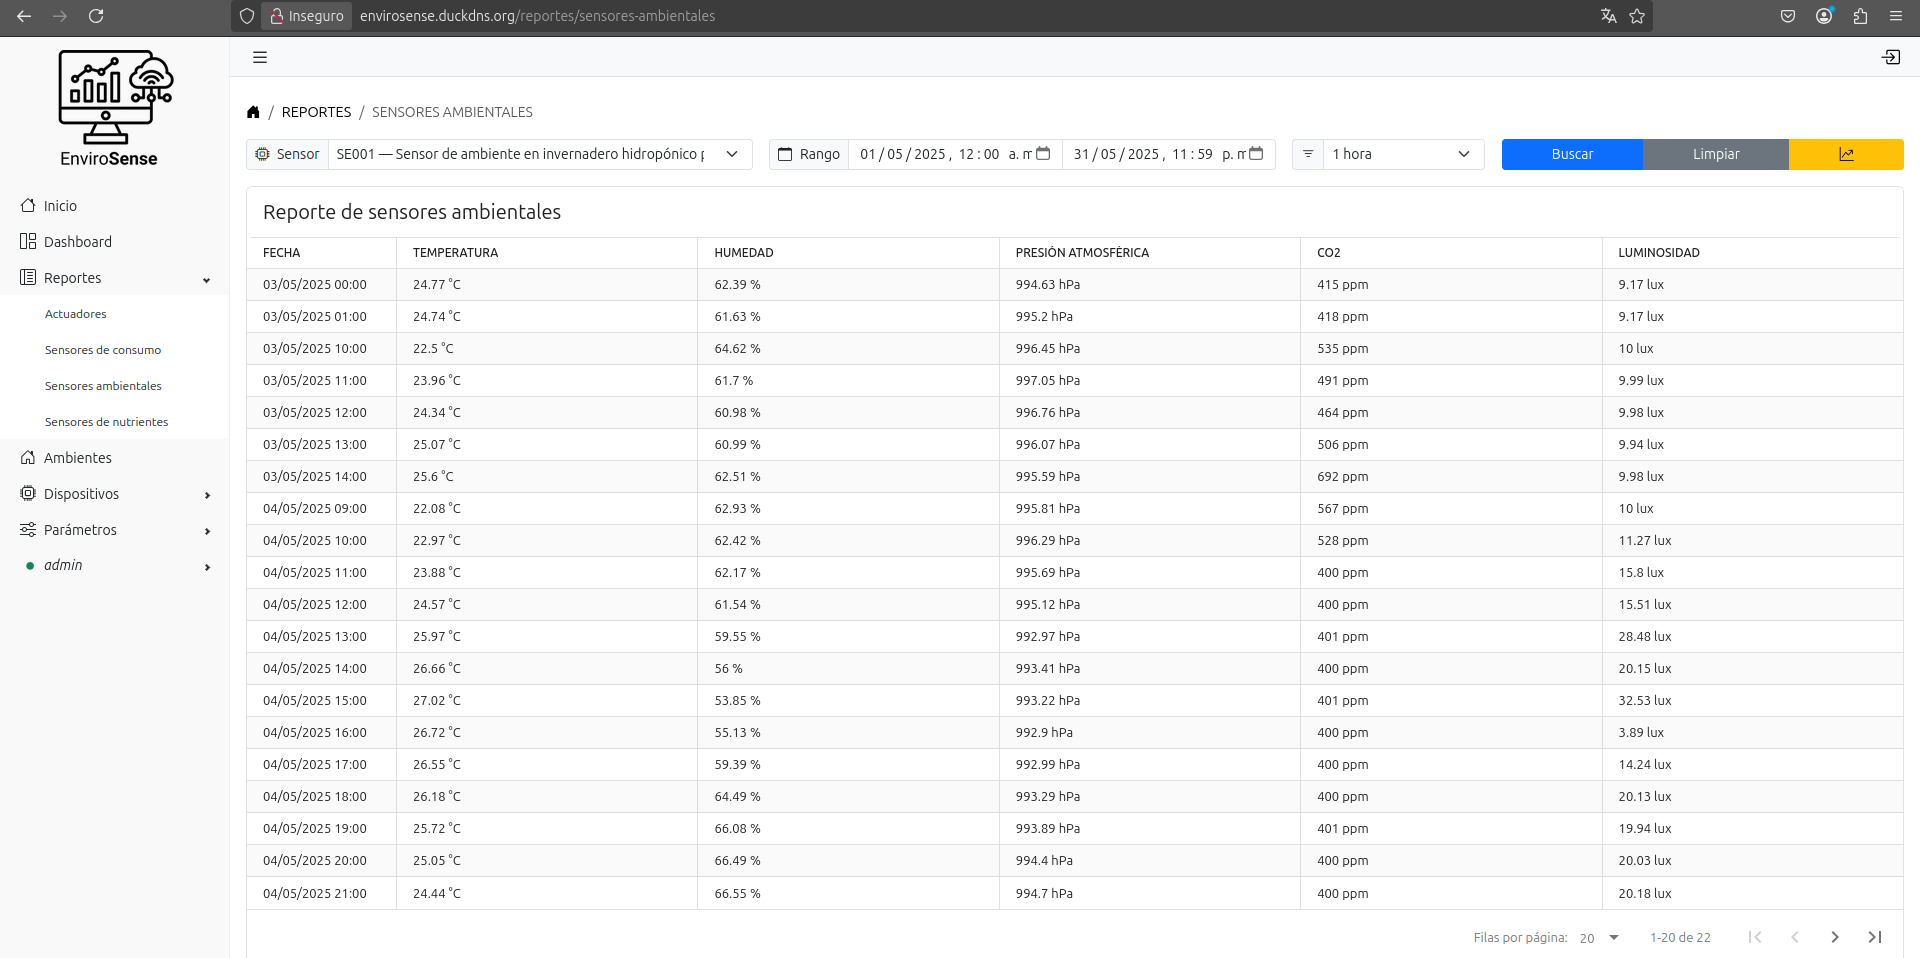
\includegraphics[width=\textwidth]{Images/45_tabla.png}
    \caption[Pruebas de funcionalidad en tablas]{Pruebas de funcionalidad en tablas.}
    \label{fig:tabla}
\end{figure}

La figura \ref{fig:grafico} muestra un ejemplo de los gráficos generados por el
sistema. Al igual que en la figura \ref{fig:tabla}, en la parte superior se
observa el formulario que permite seleccionar el sensor, el rango de fechas y
el nivel de agregación para generar el gráfico. En la parte inferior se
visualizan los gráficos generados, que representan la evolución de los datos a
lo largo del tiempo.

\begin{figure}[H]
    \centering
    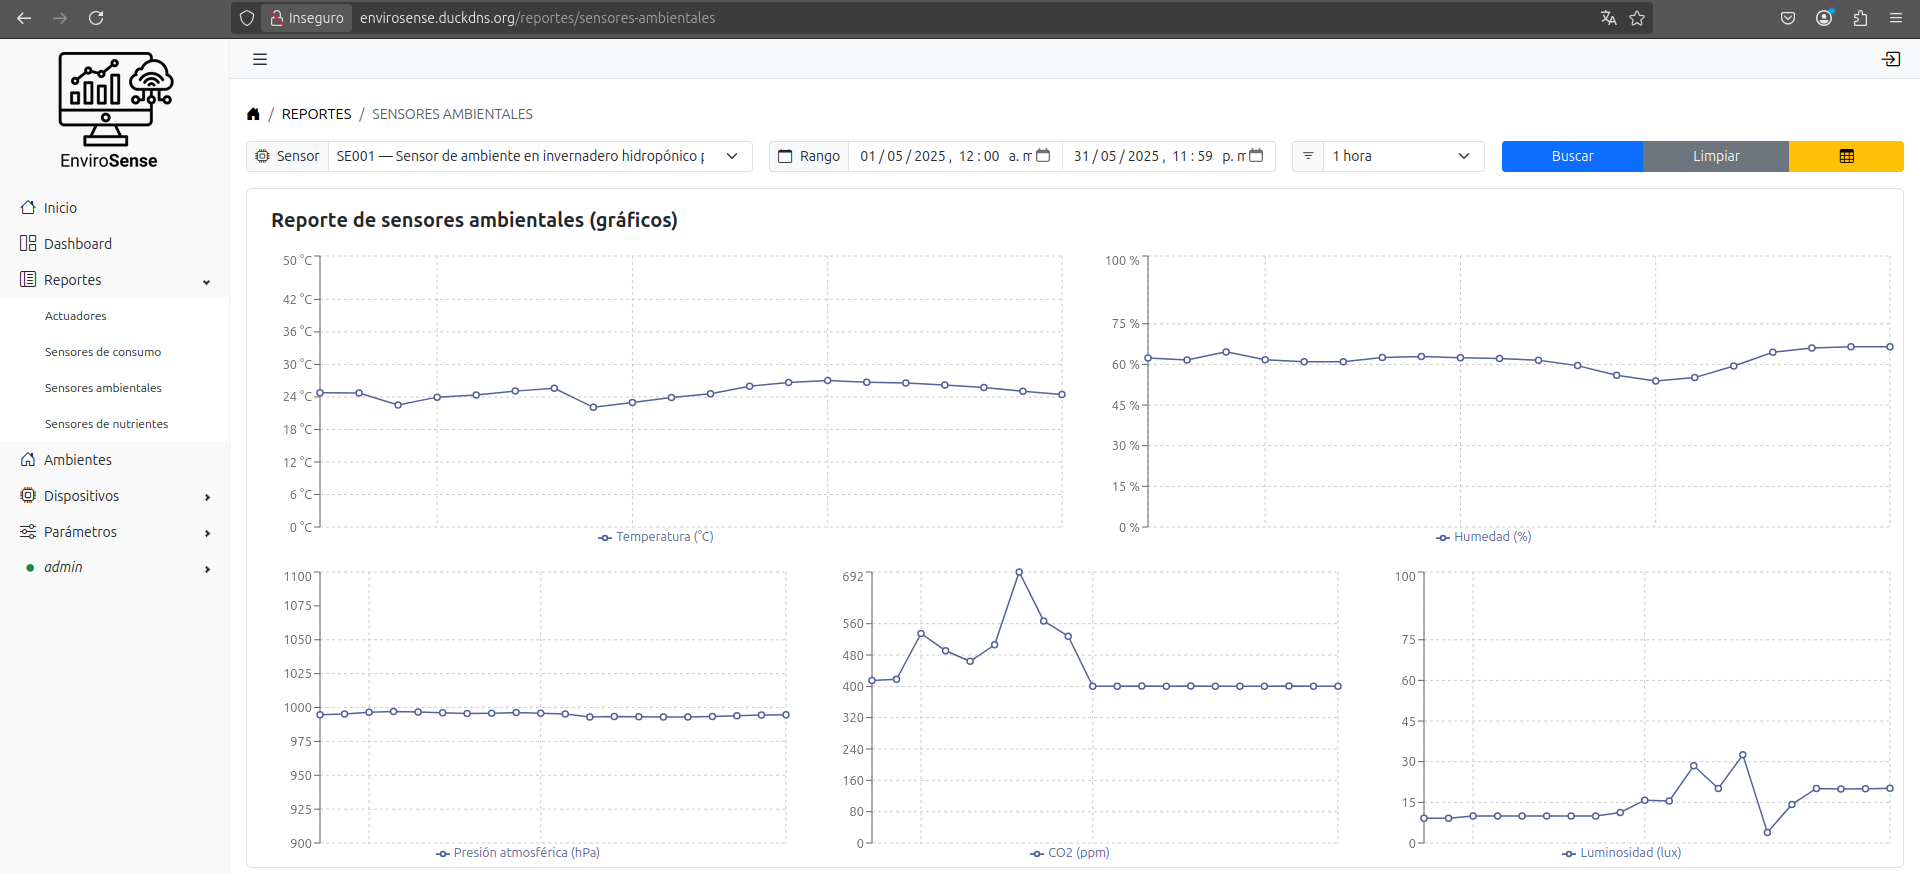
\includegraphics[width=\textwidth]{Images/46_grafico.png}
    \caption[Pruebas de funcionalidad en gráficos]{Pruebas de funcionalidad en gráficos.}
    \label{fig:grafico}
\end{figure}

\subsubsection{Validación de gráficos con WebSocket}

Se validó el funcionamiento del dashboard de monitoreo en tiempo real con
WebSocket. Se comprobó que los valores sensados se reflejaran en la interfaz
sin demoras y que los elementos visuales respondieran de forma fluida a la
transmisión continua de datos.

La figura \ref{fig:dashboard} muestra el dashboard, que incluye un menú
desplegable en la parte superior derecha para seleccionar el ambiente a
visualizar. En el centro se presentan los gráficos en tiempo real según el tipo
de sensor. En la parte inferior se visualiza el cliente WebSocket en Postman,
que confirma la correcta transmisión de datos desde el backend.

\begin{figure}[H]
    \centering
    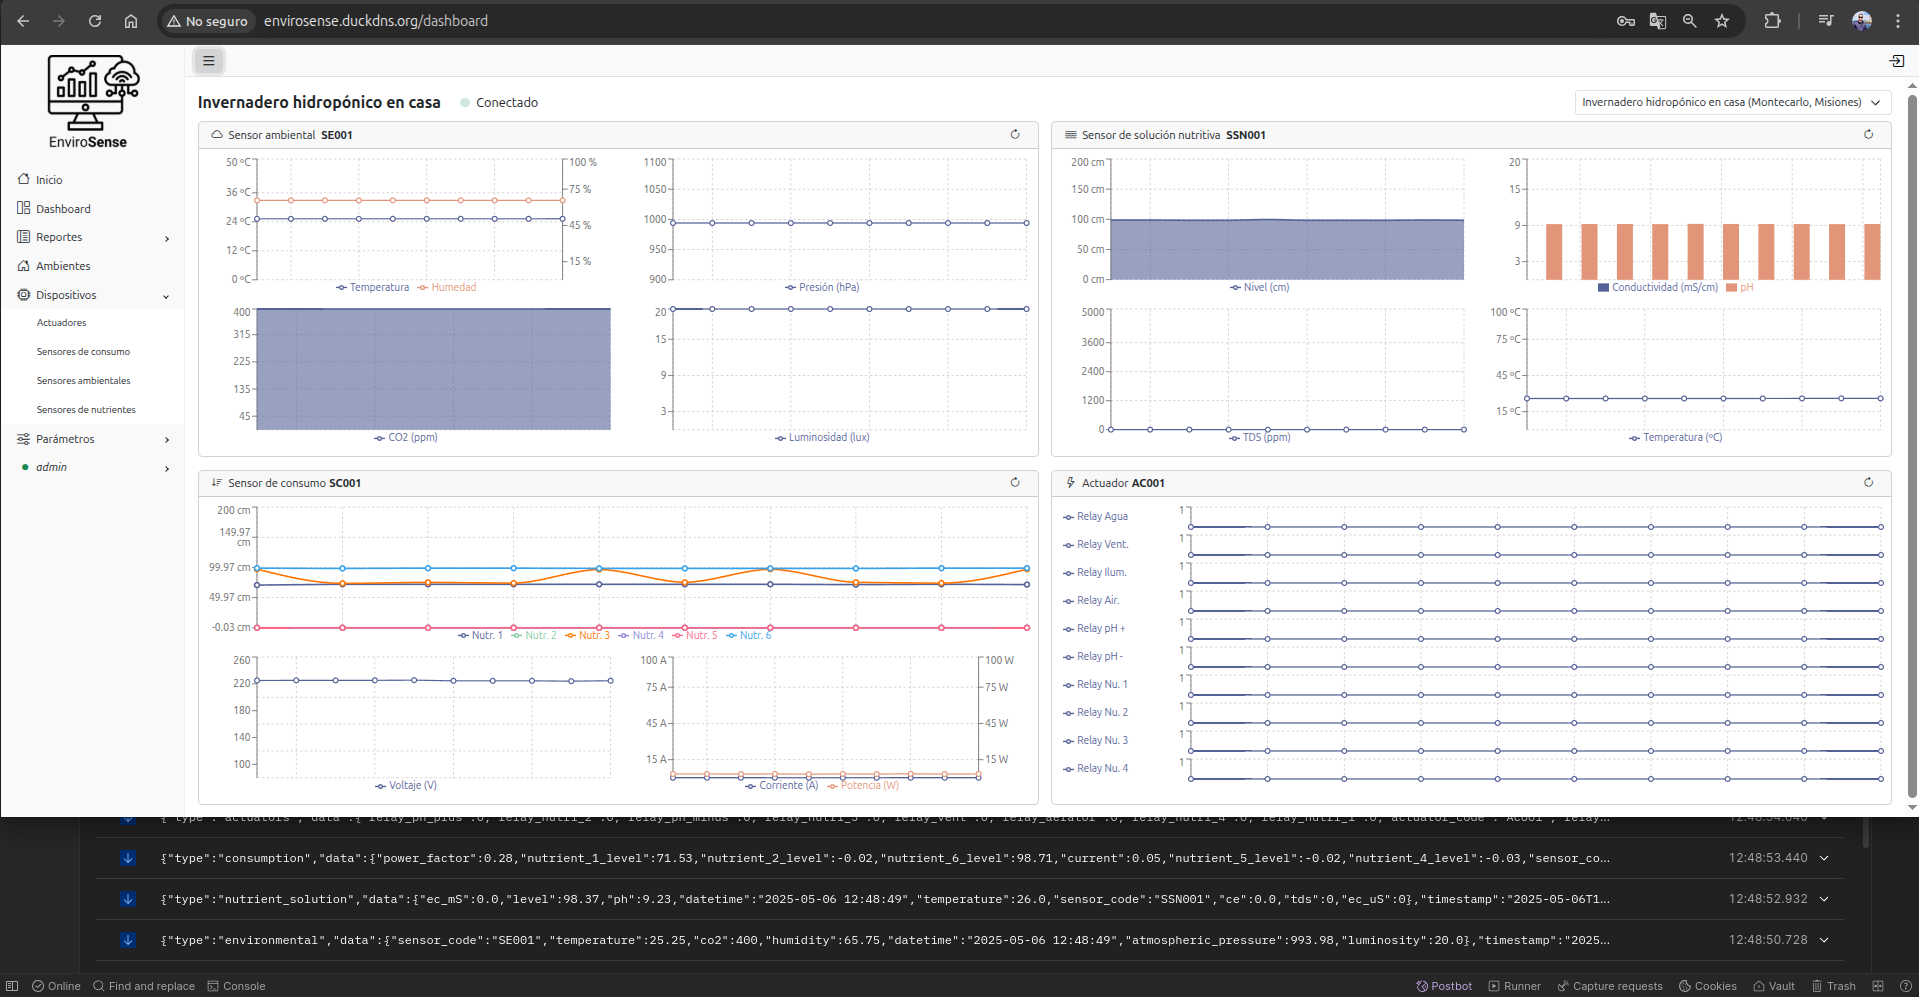
\includegraphics[width=\textwidth]{Images/47_dashboard.png}
    \caption[Pruebas de funcionalidad en el dashboard]{Pruebas de funcionalidad en el dashboard.}
    \label{fig:dashboard}
\end{figure}

\subsubsection{Pruebas de usabilidad}

Se evaluó la facilidad de uso de la interfaz y su adaptación a distintos
dispositivos, para asegurar una navegación fluida y acceso completo a las
funciones desde pantallas de diferentes tamaños.

La figura \ref{fig:responsive1} muestra un ejemplo de la interfaz de ambientes
desde un dispositivo móvil. Se verificó que todos los elementos se adaptaron
correctamente a la pantalla vertical, sin afectar su funcionalidad.

\begin{figure}[H]
    \centering
    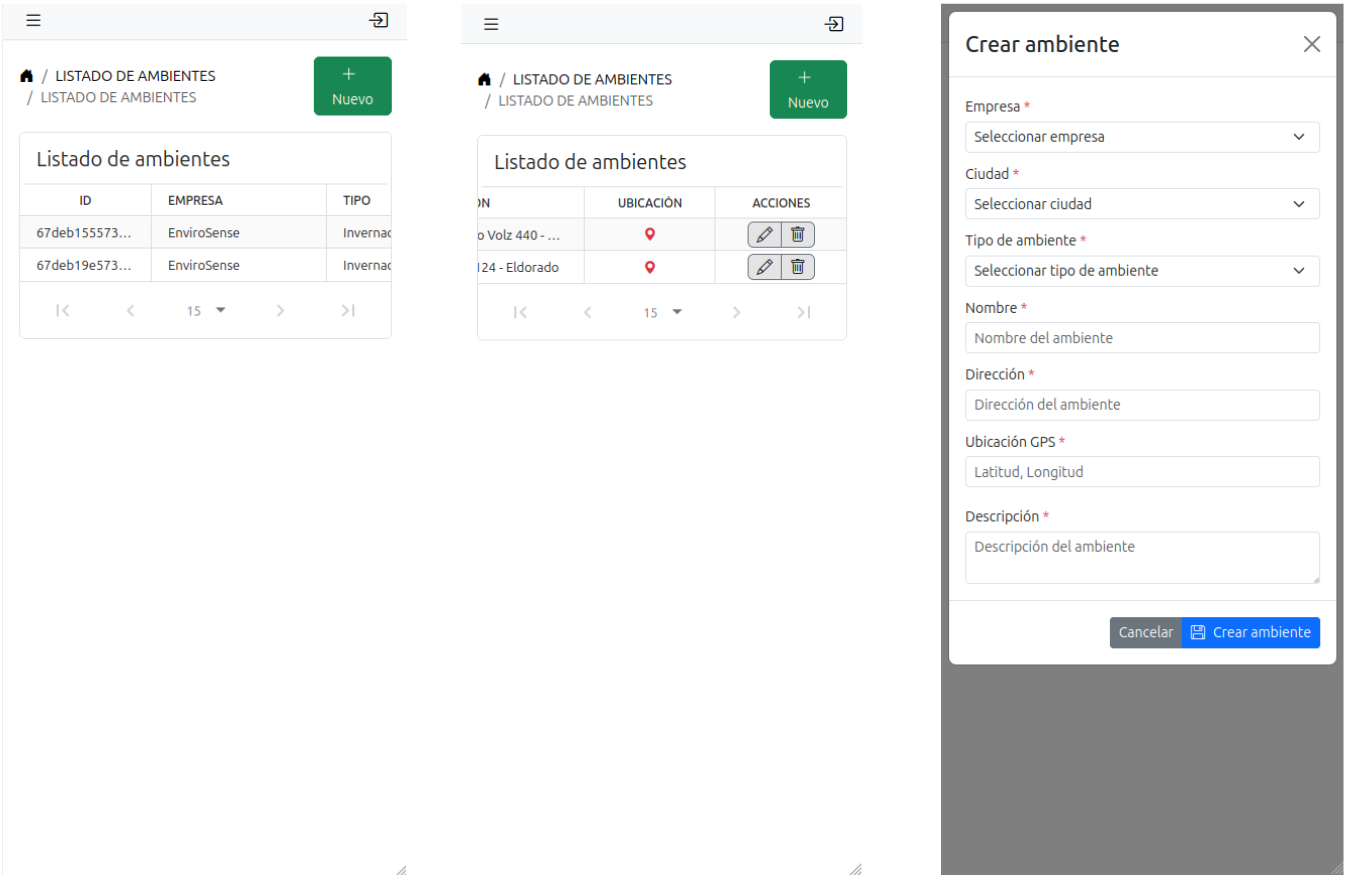
\includegraphics[width=\textwidth]{Images/49_responsive.png}
    \caption[Interfaz de ambientes en dispositivo móvil]{Interfaz de ambientes en dispositivo móvil.}
    \label{fig:responsive1}
\end{figure}

La figura \ref{fig:responsive2} presenta un listado visualizado en formato
apaisado. También en este caso los componentes de la interfaz se ajustaron de
forma adecuada, y se conservó la usabilidad.

\begin{figure}[H]
    \centering
    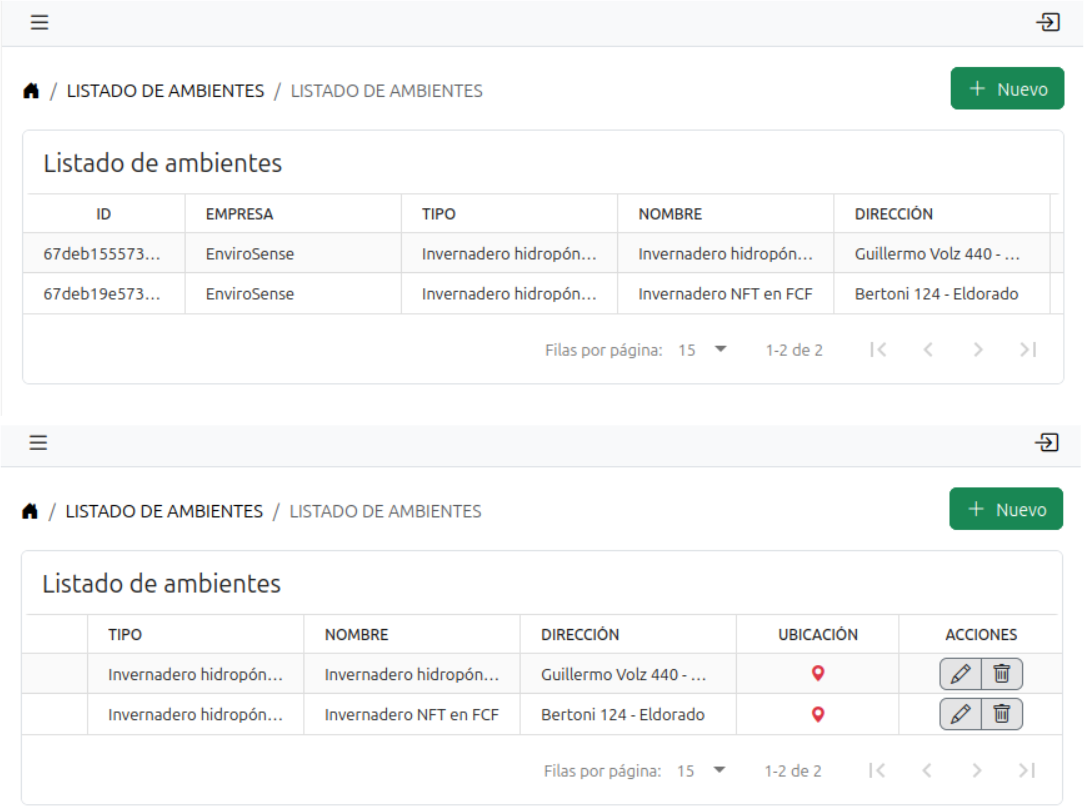
\includegraphics[width=\textwidth]{Images/50_responsive.png}
    \caption[Listado en formato apaisado desde dispositivo móvil]{Listado en formato apaisado desde dispositivo móvil.}
    \label{fig:responsive2}
\end{figure}

\section{Pruebas de componentes}

Las pruebas se realizaron con el objetivo de validar el funcionamiento de cada
componente y su integración en el entorno de prueba. Se llevaron a cabo
verificaciones individuales sobre sensores y actuadores, para evaluar la
precisión de las mediciones y la correcta respuesta ante comandos. Estas
pruebas permitieron confirmar que cada módulo cumplió con los requisitos
establecidos y operó de manera adecuada junto al resto del sistema.

Para llevarlas a cabo, los microcontroladores se conectaron a la computadora
mediante un cable USB, lo que posibilitó monitorear la salida por comunicación
serial y comprobar el comportamiento de cada módulo en forma directa.

\subsection{Pruebas de sensores}

\subsubsection{Prueba de sensor ambiental}

Se evaluaron los sensores ambientales BMP280, BH1750 y MH-Z19C, para medir la
temperatura ambiente, la humedad relativa, la presión atmosférica, el nivel de
iluminación y la concentración de $CO_2$ en el entorno de prueba.

La figura \ref{fig:medicion_sensor_ambiental} muestra un ejemplo de las
mediciones registradas por el conjunto de sensores ambientales.

\begin{figure}[H]
    \centering
    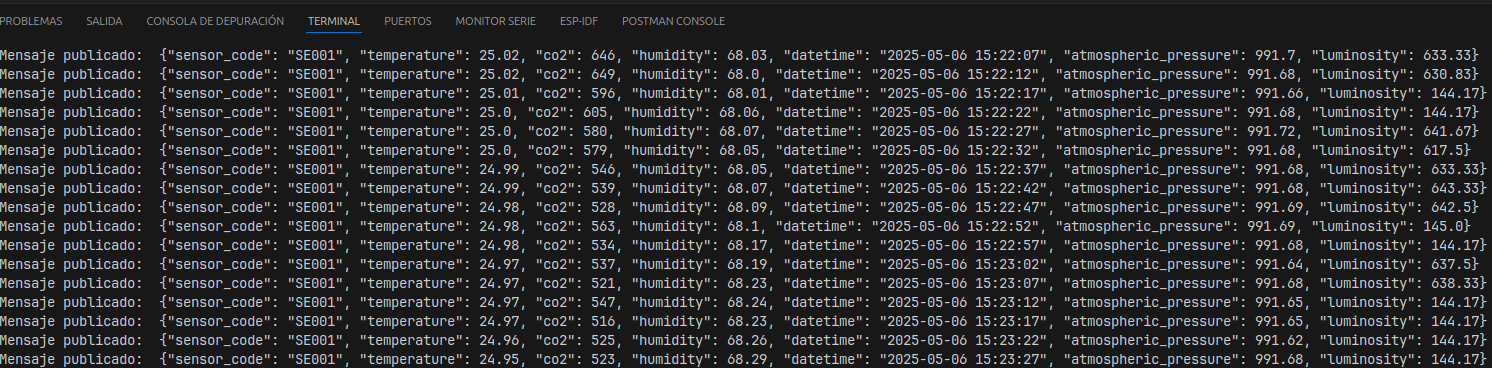
\includegraphics[width=\textwidth]{Images/51_sensor_ambiental.png}
    \caption[Pruebas de sensor ambiental]{Pruebas de sensor ambiental.}
    \label{fig:medicion_sensor_ambiental}
\end{figure}

\subsubsection{Prueba de sensor de solución nutritiva}

Se probaron sensores que permiten medir el nivel de la solución, la
temperatura, el pH, la CE y TDS de la solución nutritiva. Se utilizaron los
sensores DS18B20, PH-4502C, sensor de CE, sensor TDS y sensor ultrasónico
HC-SR04.

Para validar su funcionamiento, se realizaron dos pruebas:

\begin{itemize}
    \item Solución con agua tibia y sal: se colocaron los sensores en un recipiente con
          agua tibia y sal, con el fin de evaluar las respuestas de pH, CE y TDS ante una
          solución más concentrada.
    \item Agua potable natural: se repitió el procedimiento en un recipiente con agua
          potable natural, para comparar los resultados frente a una solución de menor
          concentración.
\end{itemize}

La figura \ref{fig:medicion_sensor_solucion} presenta los resultados obtenidos
en estas pruebas.

\begin{figure}[H]
    \centering
    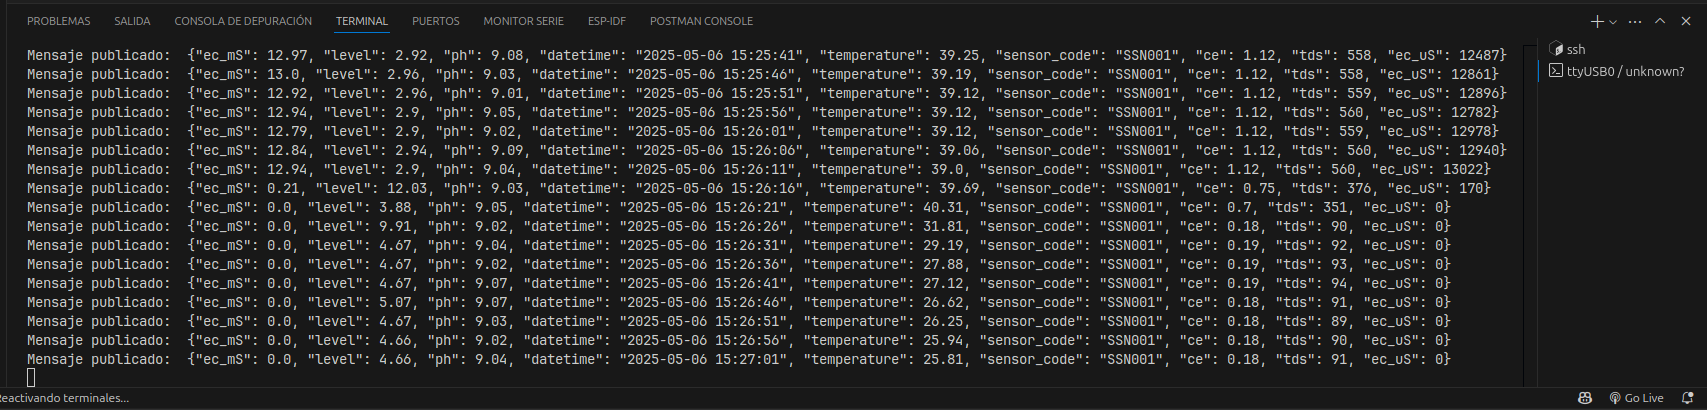
\includegraphics[width=\textwidth]{Images/52_sensor_solucion_nutritiva.png}
    \caption[Pruebas de sensor de solución nutritiva]{Pruebas de sensor de solución nutritiva.}
    \label{fig:medicion_sensor_solucion}
\end{figure}

\subsubsection{Prueba de sensor de consumos}

Se verificó el funcionamiento de los sensores destinados al monitoreo de
consumos eléctricos y del nivel en los depósitos de nutrientes. Para ello, se
utilizaron los módulos PZEM-004T y sensores ultrasónicos HC-SR04.

La figura \ref{fig:medicion_sensor_consumo} muestra un ejemplo de los datos
registrados durante las pruebas.

\begin{figure}[H]
    \centering
    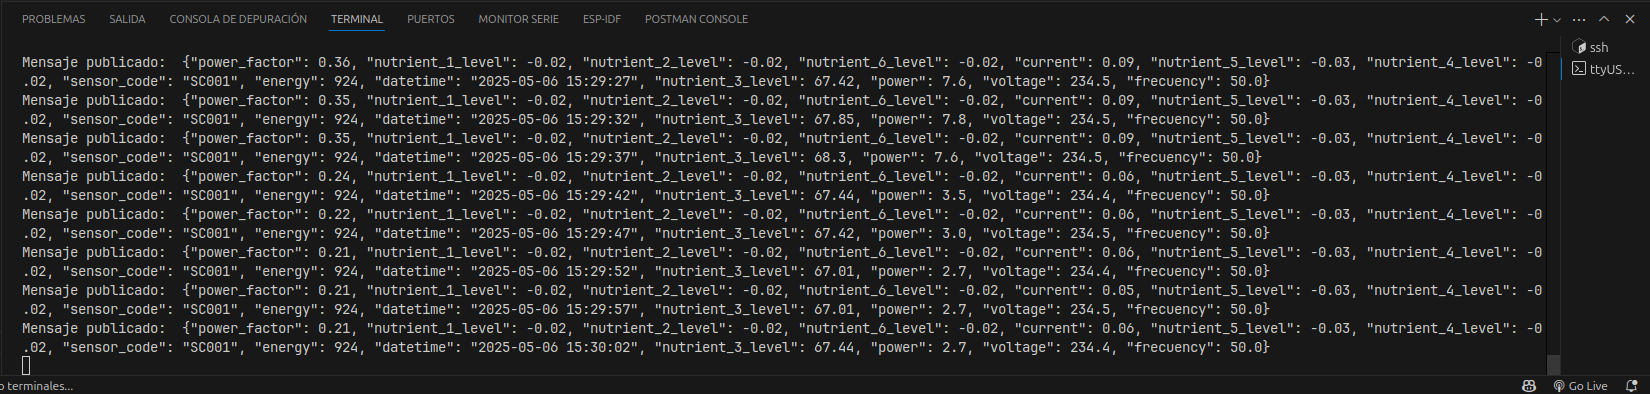
\includegraphics[width=\textwidth]{Images/53_sensor_consumos.png}
    \caption[Pruebas de sensor de consumos]{Pruebas de sensor de consumos.}
    \label{fig:medicion_sensor_consumo}
\end{figure}

\subsection{Pruebas de actuadores}

Se realizaron pruebas de los módulos de relés, que permiten activar y
desactivar dispositivos eléctricos. Se verificó su correcto funcionamiento al
activar y desactivar los relés mediante comandos enviados.

La figura \ref{fig:prueba_rele_1} muestra un ejemplo de la prueba realizada con
el módulo de relé.

\begin{figure}[H]
    \centering
    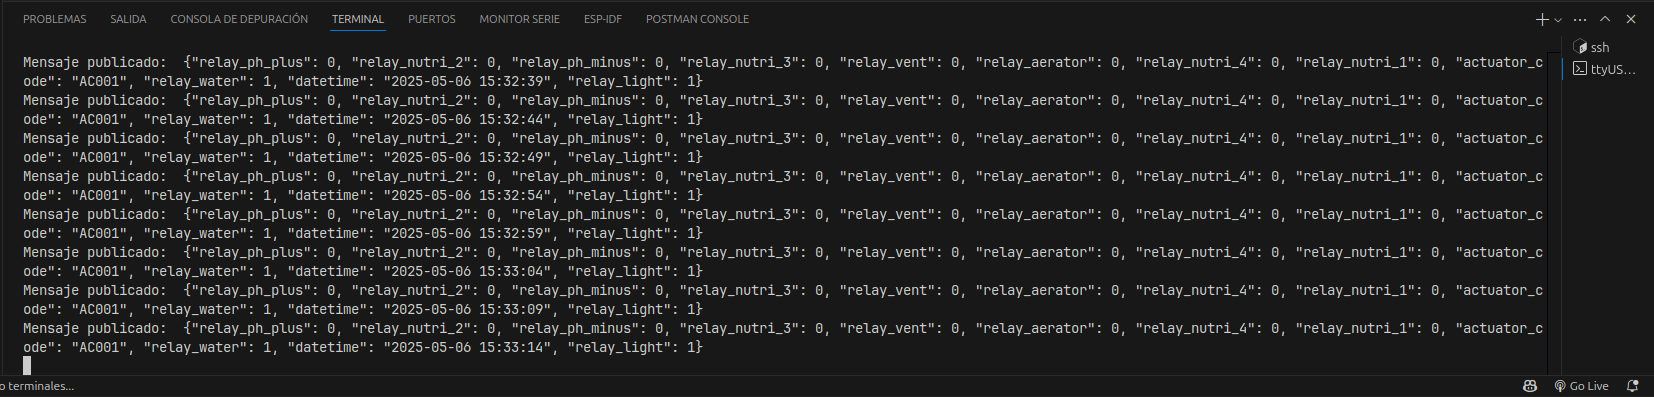
\includegraphics[width=\textwidth]{Images/54_actuadores.png}
    \caption[Pruebas de actuadores]{Pruebas de actuadores.}
    \label{fig:prueba_rele_1}
\end{figure}

La figura \ref{fig:prueba_rele_2} muestra un ejemplo de la prueba realizada con
el módulo de relé. Se verifica el encendido y apagado de los relés mediante
comandos enviados desde el microcontrolador.

\begin{figure}[H]
    \centering
    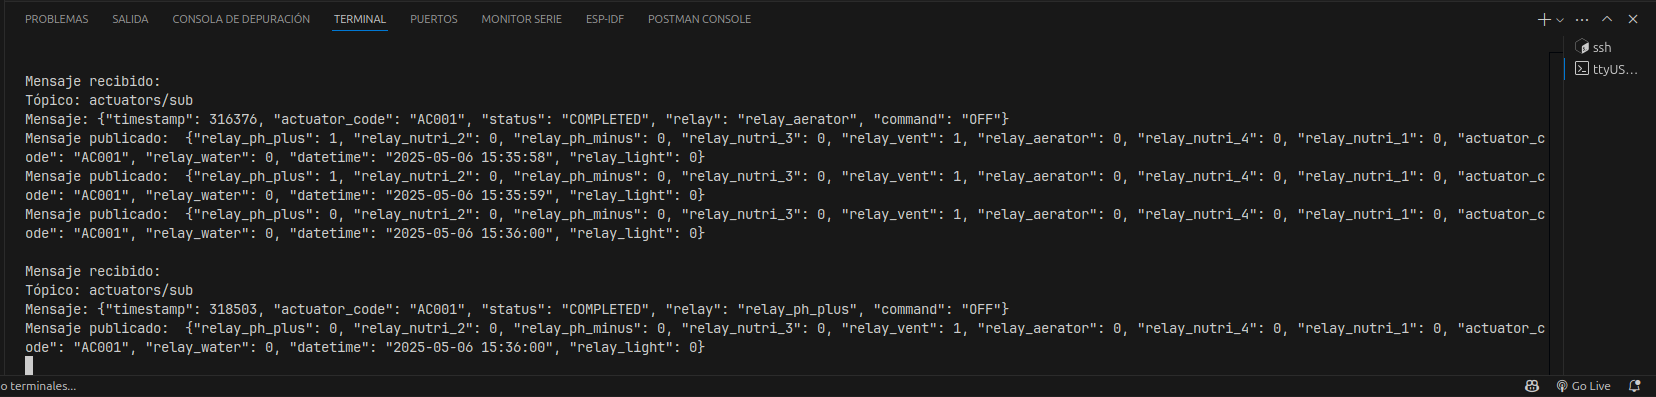
\includegraphics[width=\textwidth]{Images/54_actuadores_activacion.png}
    \caption[Pruebas de encendido de relés]{Pruebas de encendido de relés.}
    \label{fig:prueba_rele_2}
\end{figure}

\section{Pruebas de comunicación}

Las pruebas de comunicación tuvieron como objetivo validar el correcto
funcionamiento de los canales de comunicación del sistema. Se verificaron los
mensajes entre los microcontroladores y el servidor backend mediante el
protocolo MQTT, para comprobar que los mensajes enviados fueron recibidos sin
errores ni pérdidas.

Además, se evaluó la comunicación entre el backend y el frontend. Se confirmó
el procesamiento adecuado de las solicitudes de la interfaz de usuario por el
backend y la correcta presentación de las respuestas en el frontend.

Estas pruebas garantizaron la integridad del flujo de datos en toda la
arquitectura del sistema, tanto en el envío como en la recepción de
información.

\subsection{Pruebas en sensor ambiental}

La figura \ref{fig:prueba_mqtt_sensor_ambiental_1} muestra una prueba en la que
se envió un mensaje MQTT al sensor ambiental para modificar el intervalo de
envío de datos a 45 segundos.

\begin{figure}[H]
    \centering
    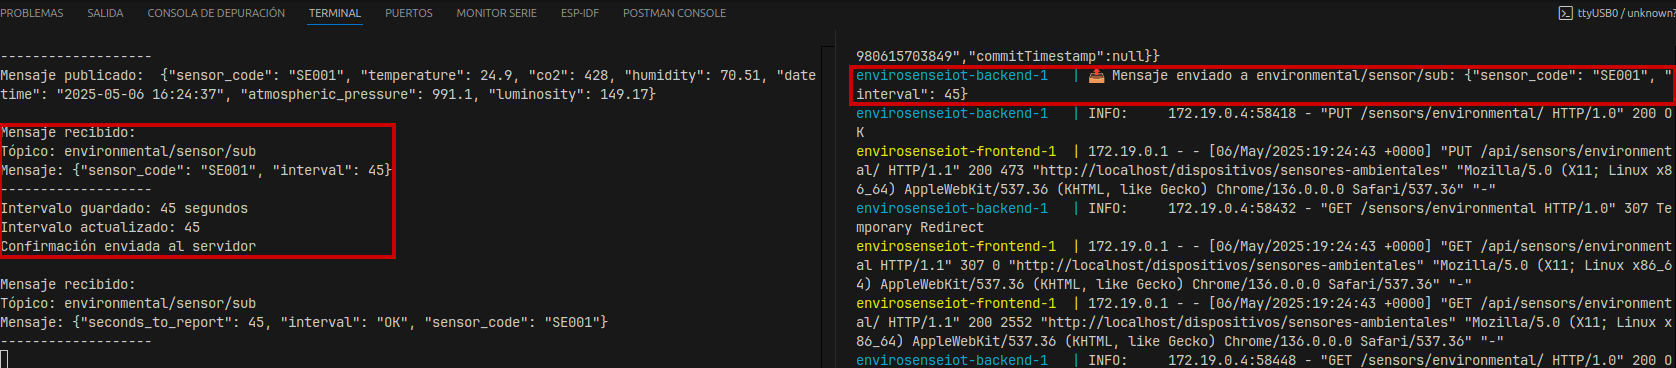
\includegraphics[width=\textwidth]{Images/55_prueba_mqtt_sensor_ambiental_1.png}
    \caption[Pruebas de comunicación con sensor ambiental]{Pruebas de comunicación con sensor ambiental.}
    \label{fig:prueba_mqtt_sensor_ambiental_1}
\end{figure}

En la figura \ref{fig:prueba_mqtt_sensor_ambiental_2} se observa una prueba en
la que se solicitó al sensor enviar sus datos al backend. El dispositivo
procesó la solicitud y respondió con los valores capturados, los cuales fueron
recibidos correctamente y almacenados en la base de datos.

\begin{figure}[H]
    \centering
    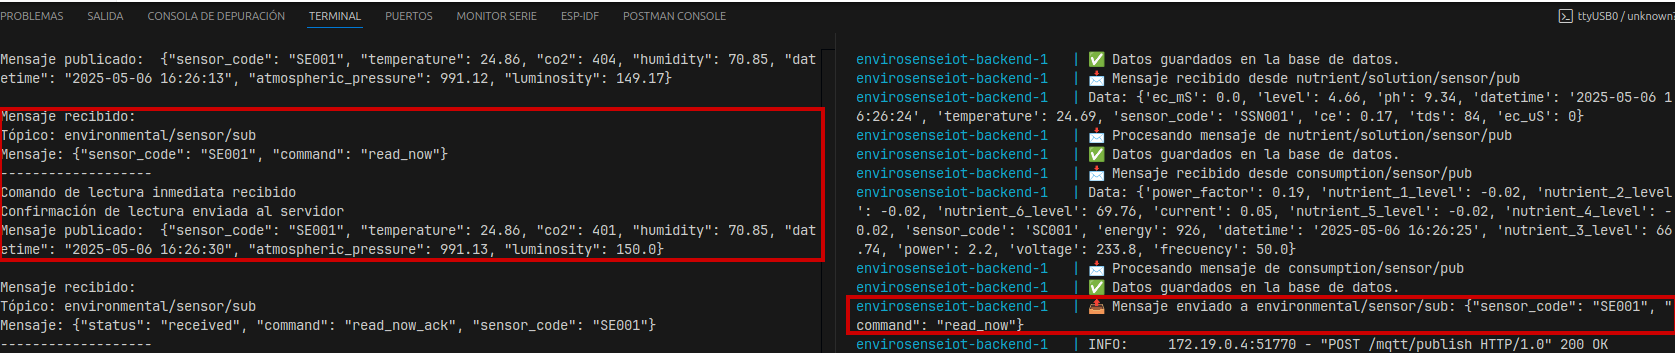
\includegraphics[width=\textwidth]{Images/55_prueba_mqtt_sensor_ambiental_2.png}
    \caption[Pruebas de comunicación con sensor ambiental]{Pruebas de comunicación con sensor ambiental.}
    \label{fig:prueba_mqtt_sensor_ambiental_2}
\end{figure}

\subsection{Pruebas en sensor de consumos}

La figura \ref{fig:prueba_mqtt_sensor_consumos_1} presenta una prueba en la que
se envió un mensaje MQTT al sensor de consumos para establecer un nuevo
intervalo de transmisión de datos de 45 segundos.

\begin{figure}[H]
    \centering
    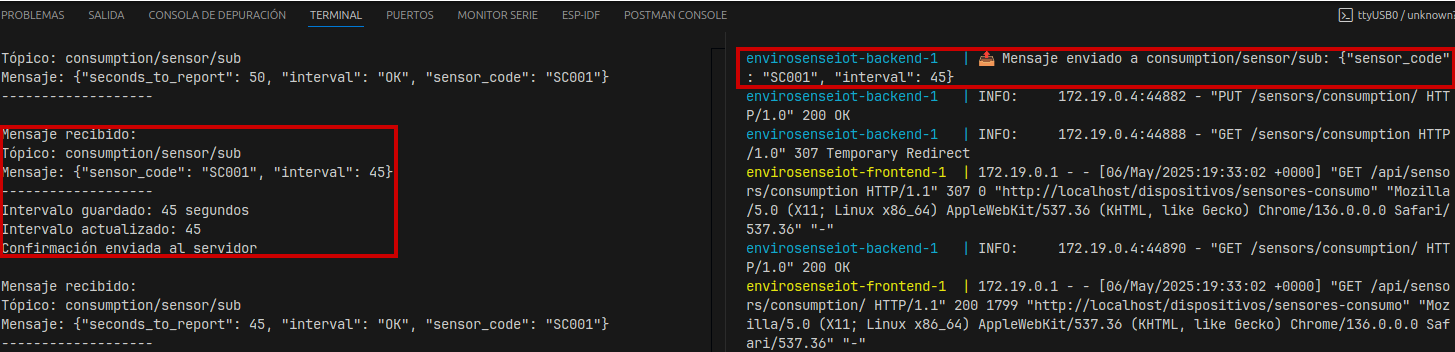
\includegraphics[width=\textwidth]{Images/56_prueba_mqtt_sensor_consumos_1.png}
    \caption[Pruebas de comunicación con sensor de consumos]{Pruebas de comunicación con sensor de consumos.}
    \label{fig:prueba_mqtt_sensor_consumos_1}
\end{figure}

La figura \ref{fig:prueba_mqtt_sensor_consumos_2} ilustra una prueba en la que
se solicitó al sensor de consumos transmitir sus mediciones al backend. El
sensor respondió con los datos requeridos, que fueron correctamente registrados
en la base de datos.

\begin{figure}[H]
    \centering
    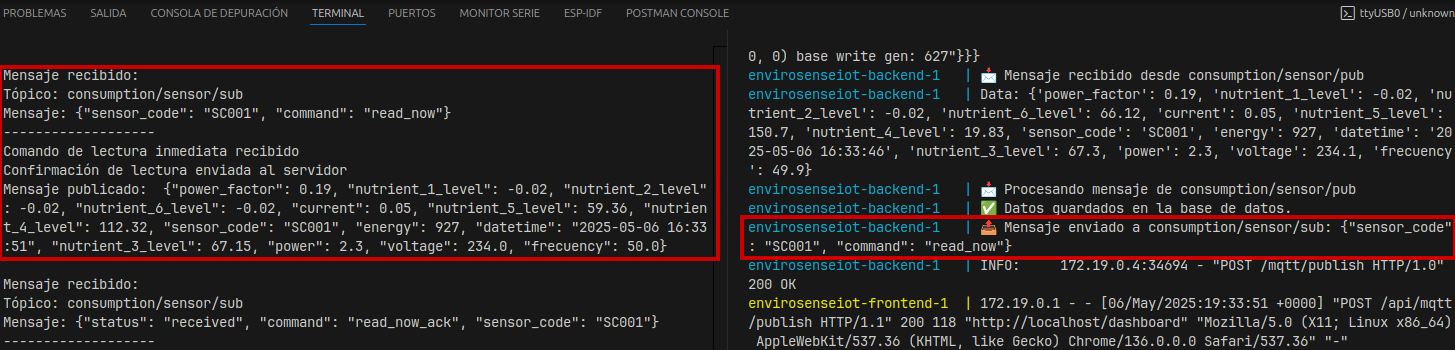
\includegraphics[width=\textwidth]{Images/56_prueba_mqtt_sensor_consumos_2.png}
    \caption[Pruebas de comunicación con sensor de consumos]{Pruebas de comunicación con sensor de consumos.}
    \label{fig:prueba_mqtt_sensor_consumos_2}
\end{figure}

\subsection{Pruebas en sensor de solución nutritiva}

La figura \ref{fig:prueba_mqtt_sensor_solucion_nutritiva_1} presenta una prueba
en la que se envió un mensaje MQTT al sensor de solución nutritiva para fijar
un nuevo intervalo de transmisión de datos en 45 segundos.

\begin{figure}[H]
    \centering
    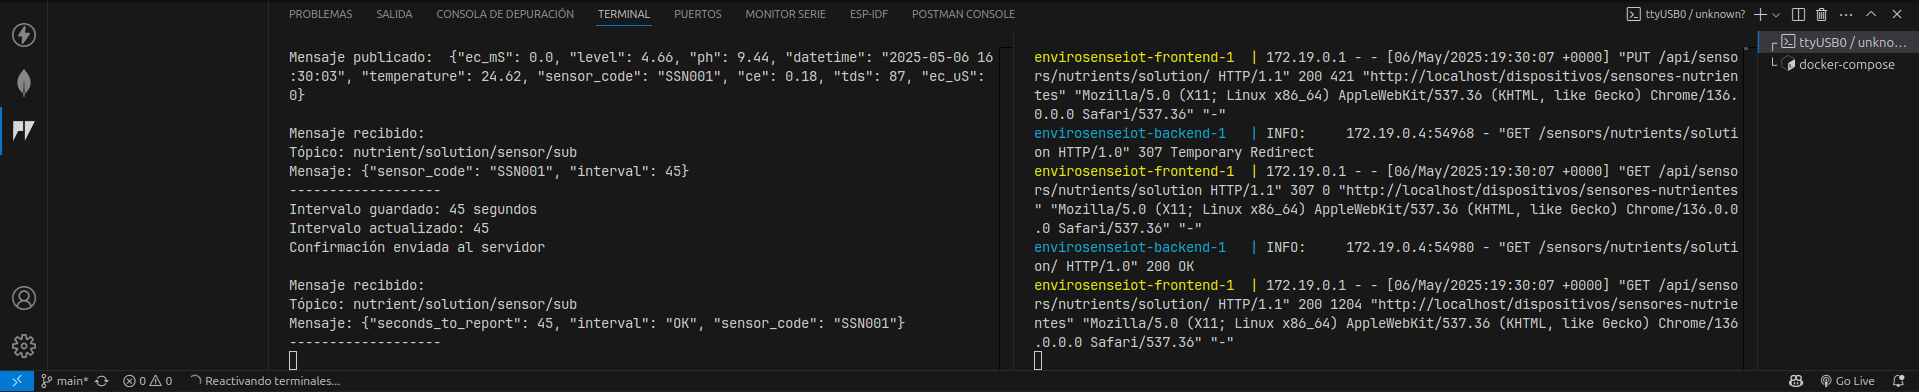
\includegraphics[width=\textwidth]{Images/57_prueba_mqtt_sensor_solucion_nutritiva_1.png}
    \caption[Pruebas de comunicación con sensor de solución nutritiva]{Pruebas de comunicación con sensor de solución nutritiva.}
    \label{fig:prueba_mqtt_sensor_solucion_nutritiva_1}
\end{figure}

La figura \ref{fig:prueba_mqtt_sensor_solucion_nutritiva_2} evidencia una
prueba en la que se solicitó al sensor de solución nutritiva la transmisión de
los valores de nivel, temperatura, pH, CE y TDS al backend. El sensor respondió
con los datos requeridos, los cuales se registraron correctamente en la base de
datos.

\begin{figure}[H]
    \centering
    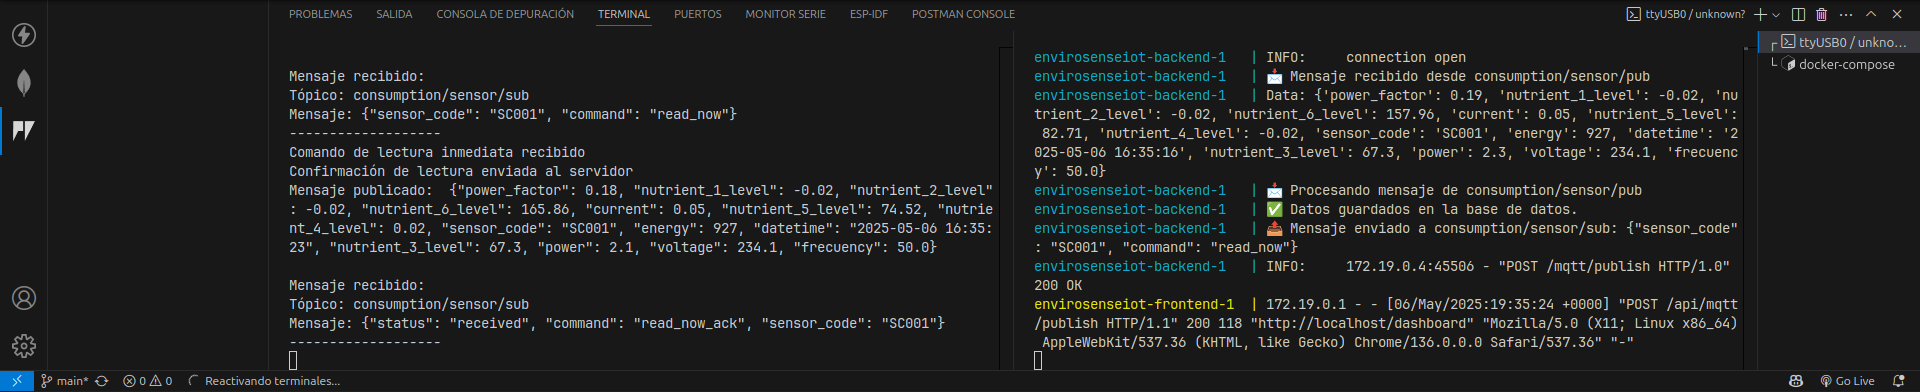
\includegraphics[width=\textwidth]{Images/57_prueba_mqtt_sensor_solucion_nutritiva_2.png}
    \caption[Pruebas de comunicación con sensor de solución nutritiva]{Pruebas de comunicación con sensor de solución nutritiva.}
    \label{fig:prueba_mqtt_sensor_solucion_nutritiva_2}
\end{figure}

\subsection{Pruebas de comunicación en el actuador}

La figura \ref{fig:prueba_mqtt_actuador_1} muestra una prueba en la que se
envió un mensaje MQTT al actuador para establecer un nuevo intervalo de
transmisión de datos de 45 segundos.

\begin{figure}[H]
    \centering
    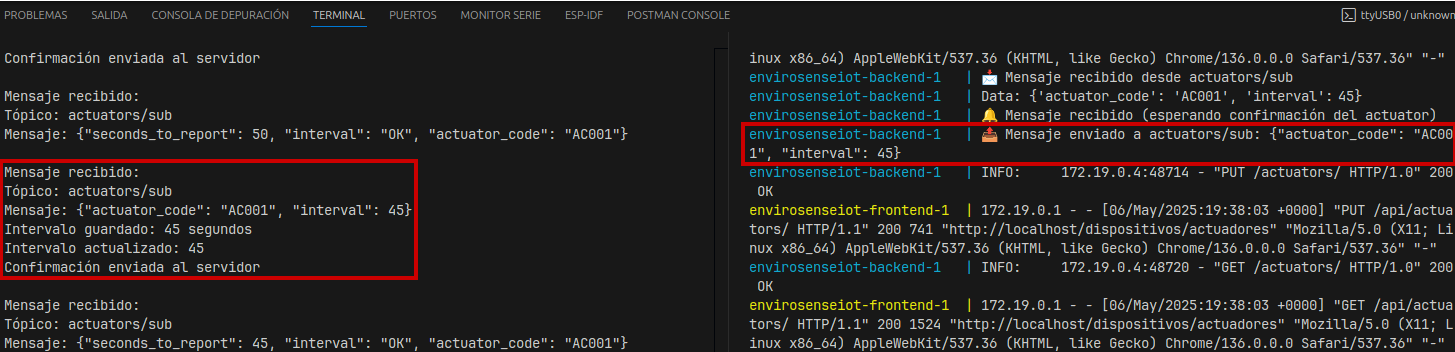
\includegraphics[width=\textwidth]{Images/58_prueba_mqtt_actuador_1.png}
    \caption[Pruebas de comunicación con actuador]{Pruebas de comunicación con actuador.}
    \label{fig:prueba_mqtt_actuador_1}
\end{figure}

La figura \ref{fig:prueba_mqtt_actuador_2} ilustra una prueba en la que se
solicitó al actuador que transmitiera el estado de los relés al backend. El
actuador respondió con los valores de cada relé, que fueron correctamente
registrados en la base de datos.

\begin{figure}[H]
    \centering
    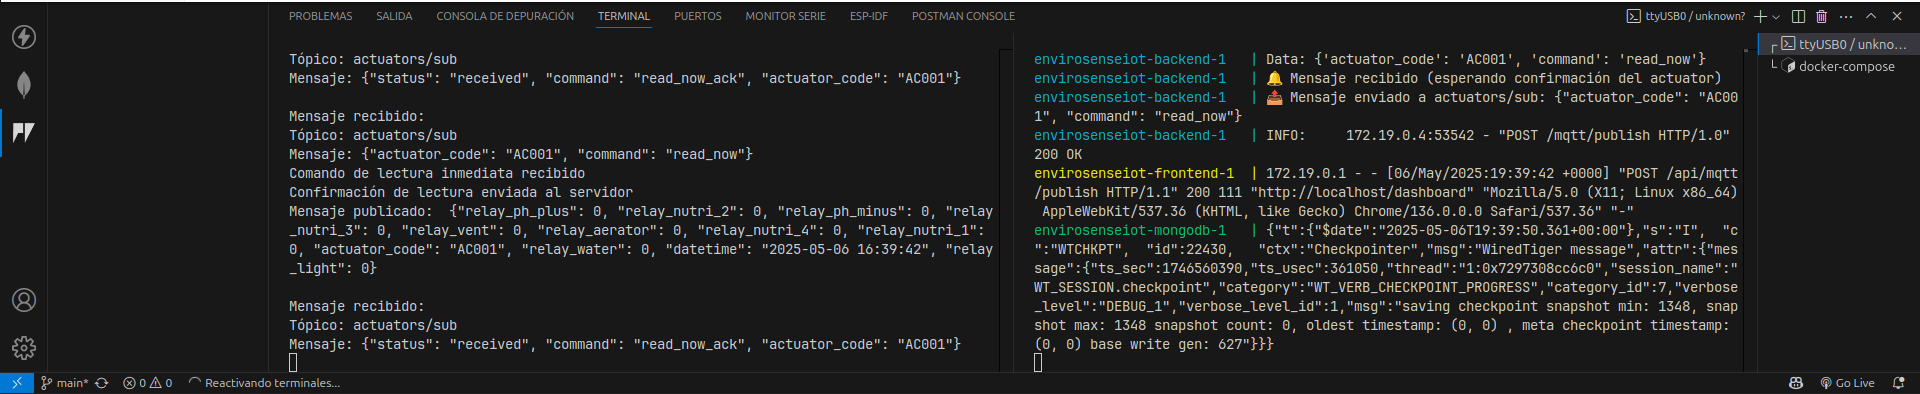
\includegraphics[width=\textwidth]{Images/58_prueba_mqtt_actuador_2.png}
    \caption[Pruebas de comunicación con actuador]{Pruebas de comunicación con actuador.}
    \label{fig:prueba_mqtt_actuador_2}
\end{figure}

La figura \ref{fig:prueba_mqtt_actuador_3} permite visualizar una prueba en la
que se envió un mensaje MQTT al actuador para activar el relé correspondiente a
la bomba de agua durante cinco segundos. Al recibir el comando, el actuador
ejecutó la acción y envió un mensaje con el estado de los relés. Finalizado el
tiempo, transmitió un nuevo mensaje con el estado actualizado, y la
confirmación de que la operación ha sido completada correctamente.

\begin{figure}[H]
    \centering
    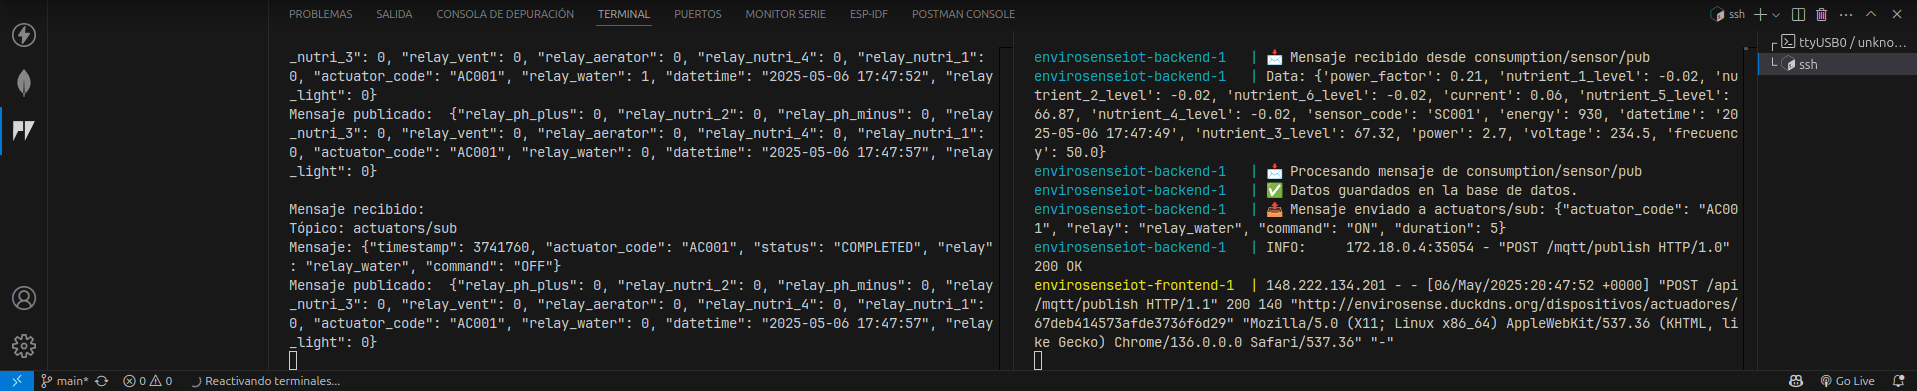
\includegraphics[width=\textwidth]{Images/58_prueba_mqtt_actuador_3.png}
    \caption[Pruebas de comunicación con actuador]{Pruebas de comunicación con actuador.}
    \label{fig:prueba_mqtt_actuador_3}
\end{figure}

\section{Prueba integral del sistema}

Esta prueba tuvo como objetivo validar el funcionamiento completo del sistema,
para asegurar la correcta interacción entre todos los componentes: frontend,
backend y dispositivos conectados. Se buscó verificar la secuencia de
comunicación entre las distintas partes sin interrupciones ni errores.

La prueba comenzó en el frontend, donde se seleccionó un actuador y se accedió
a su detalle. A continuación, se activó el relé correspondiente a la bomba de
agua por un período de 30 segundos.

La figura \ref{fig:prueba_integral_1} muestra la interfaz del frontend al
momento de ejecutar la orden de activación del relé.

\begin{figure}[H]
    \centering
    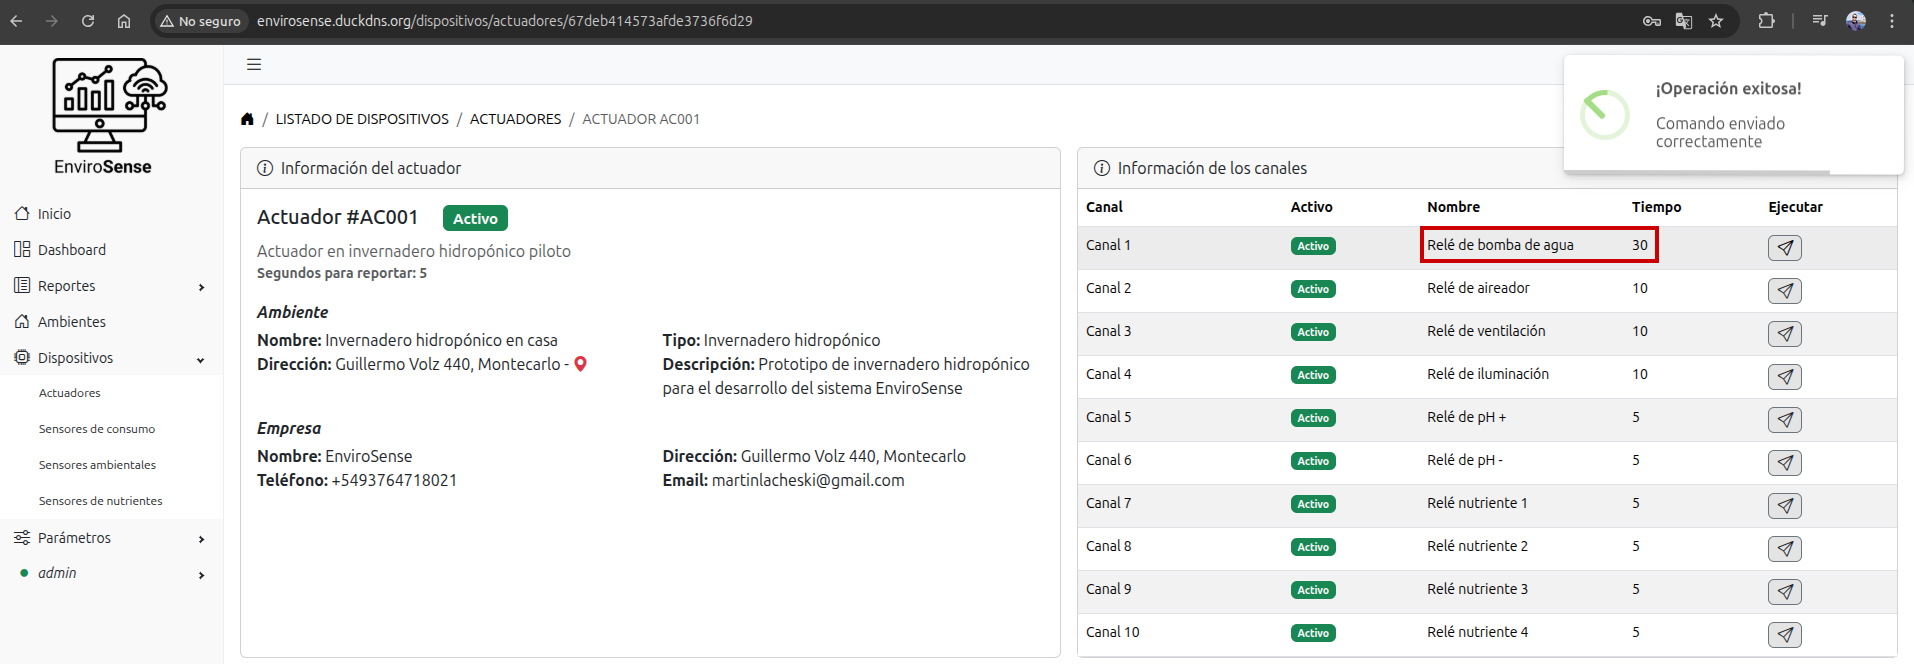
\includegraphics[width=\textwidth]{Images/59_prueba_integral_1.png}
    \caption[Envío de comando de activación al microcontrolador]{Envío de comando de activación al microcontrolador.}
    \label{fig:prueba_integral_1}
\end{figure}

Al hacer clic en la interfaz, el frontend envió una petición HTTP tipo POST al
backend. La figura \ref{fig:prueba_integral_2} muestra la salida por consola
del frontend, donde se visualiza el envío de dicha solicitud.

\begin{figure}[H]
    \centering
    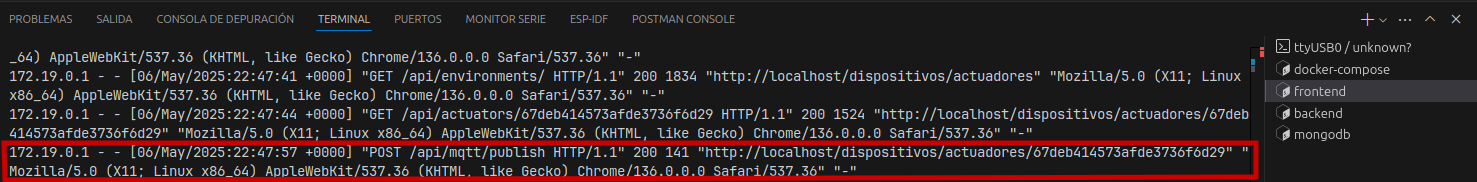
\includegraphics[width=\textwidth]{Images/59_prueba_integral_2.png}
    \caption[Salida por consola del frontend]{Salida por consola del frontend.}
    \label{fig:prueba_integral_2}
\end{figure}

El backend recibió esta solicitud, la procesó y publicó un mensaje MQTT en el
tópico correspondiente al microcontrolador. Luego respondió al frontend con un
estado 200 OK, para indicar que la acción fue ejecutada correctamente.

En la figura \ref{fig:prueba_integral_3} se observa la salida por consola del
backend, el registro de la recepción de la solicitud, el envío del mensaje MQTT
y la respuesta al frontend.

\begin{figure}[H]
    \centering
    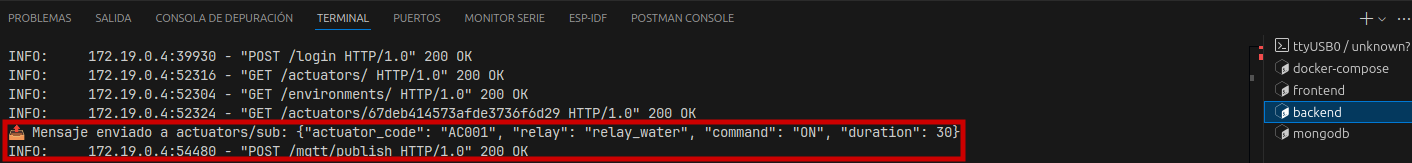
\includegraphics[width=\textwidth]{Images/59_prueba_integral_3.png}
    \caption[Salida por consola del backend]{Salida por consola del backend.}
    \label{fig:prueba_integral_3}
\end{figure}

El microcontrolador, suscripto al tópico correspondiente, recibió el mensaje,
con el comando, el canal correspondiente y el tiempo de activación. Procesó la
información y activó el relé de la bomba de agua.

Luego, envió una respuesta al backend con el estado actualizado de los relés.
Una vez transcurrido el tiempo programado, volvió a enviar un nuevo mensaje
para indicar que la operación fue completada con éxito.

La figura \ref{fig:prueba_integral_4} muestra la consola del microcontrolador,
donde se registra la recepción del mensaje, la activación del relé y la
respuesta enviada.

\begin{figure}[H]
    \centering
    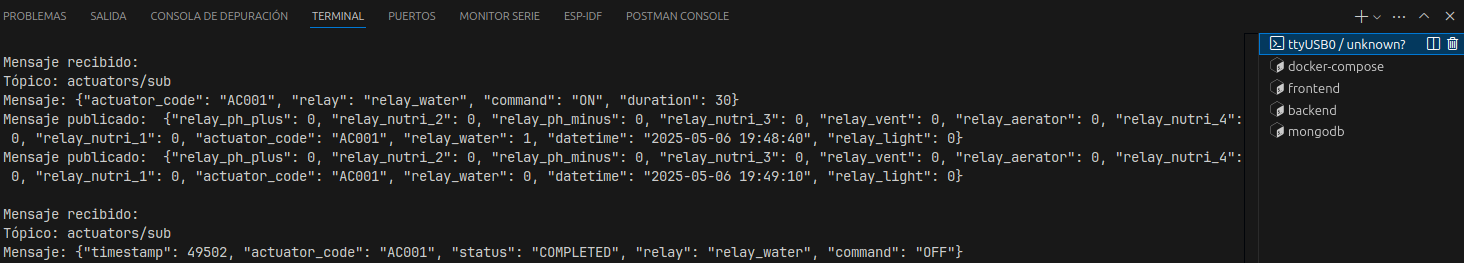
\includegraphics[width=\textwidth]{Images/59_prueba_integral_4.png}
    \caption[Salida por consola del microcontrolador]{Salida por consola del microcontrolador.}
    \label{fig:prueba_integral_4}
\end{figure}

Posteriormente, el backend recibió el mensaje del microcontrolador y lo
almacenó en la base de datos.

La figura \ref{fig:prueba_integral_5} muestra la salida por consola del
backend, donde se observa la recepción del mensaje del microcontrolador y el
almacenamiento en la base de datos.

\begin{figure}[H]
    \centering
    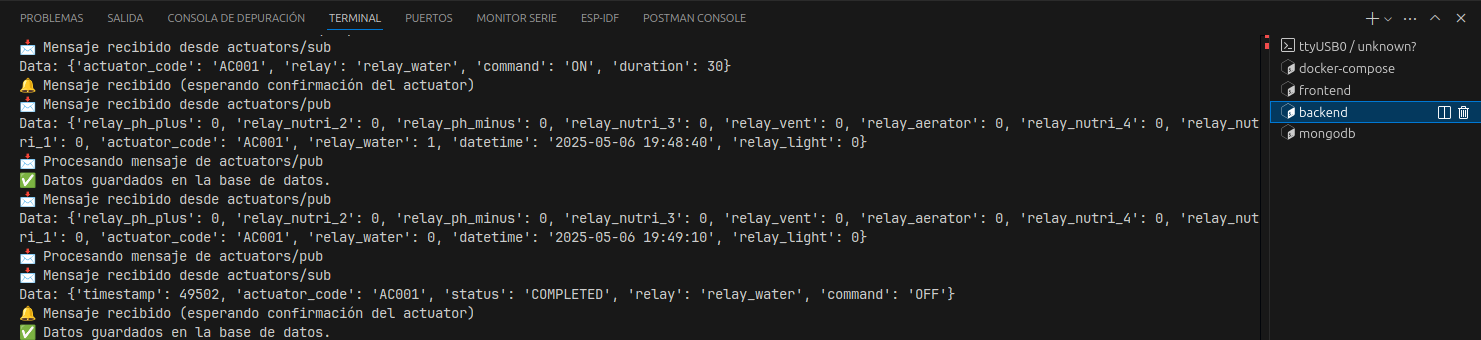
\includegraphics[width=\textwidth]{Images/59_prueba_integral_5.png}
    \caption[Salida por consola del backend]{Salida por consola del backend.}
    \label{fig:prueba_integral_5}
\end{figure}

Para validar el almacenamiento, se utilizó MongoDB Compass. En la figura
\ref{fig:prueba_integral_6} se muestra la colección \texttt{ActuatorData},
donde se evidencia el registro del estado de los relés y la marca temporal de
la operación, para reflejar el encendido y apagado de la bomba de agua.

\begin{figure}[H]
    \centering
    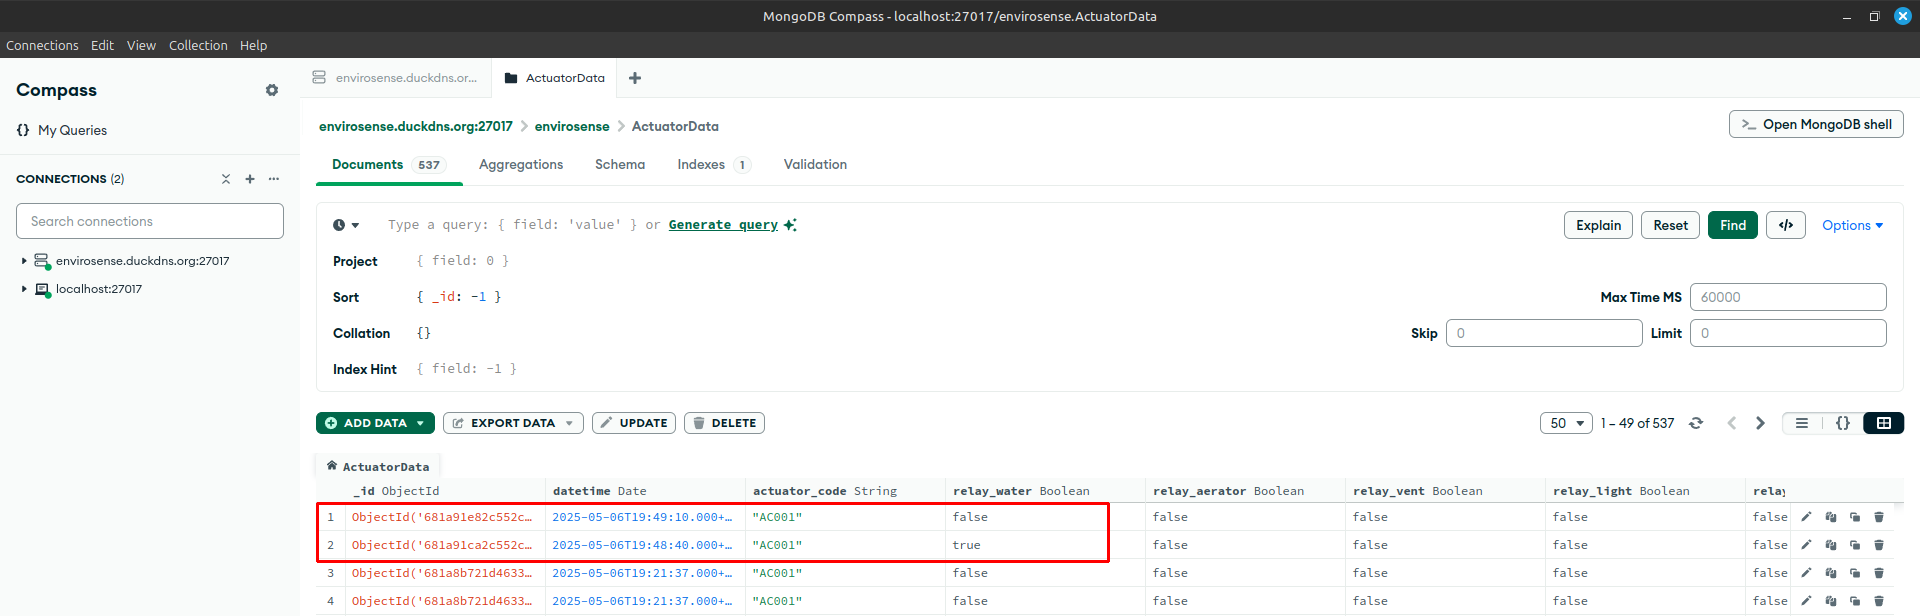
\includegraphics[width=\textwidth]{Images/59_prueba_integral_6.png}
    \caption[Verificación de persistencia en MongoDB Compass]{Verificación de persistencia en MongoDB Compass.}
    \label{fig:prueba_integral_6}
\end{figure}

Finalmente, el backend, envía un mensaje a todos los clientes conectados
mediante WebSocket, para notificar la actualización del estado de los relés. El
cliente recibe el mensaje y actualiza la interfaz, para reflejar el nuevo
estado de los relés.

La figura \ref{fig:prueba_integral_7} muestra el dashboard del frontend, donde
se visualiza el estado actualizado de los relés, junto con la hora del sistema
como referencia.

\begin{figure}[H]
    \centering
    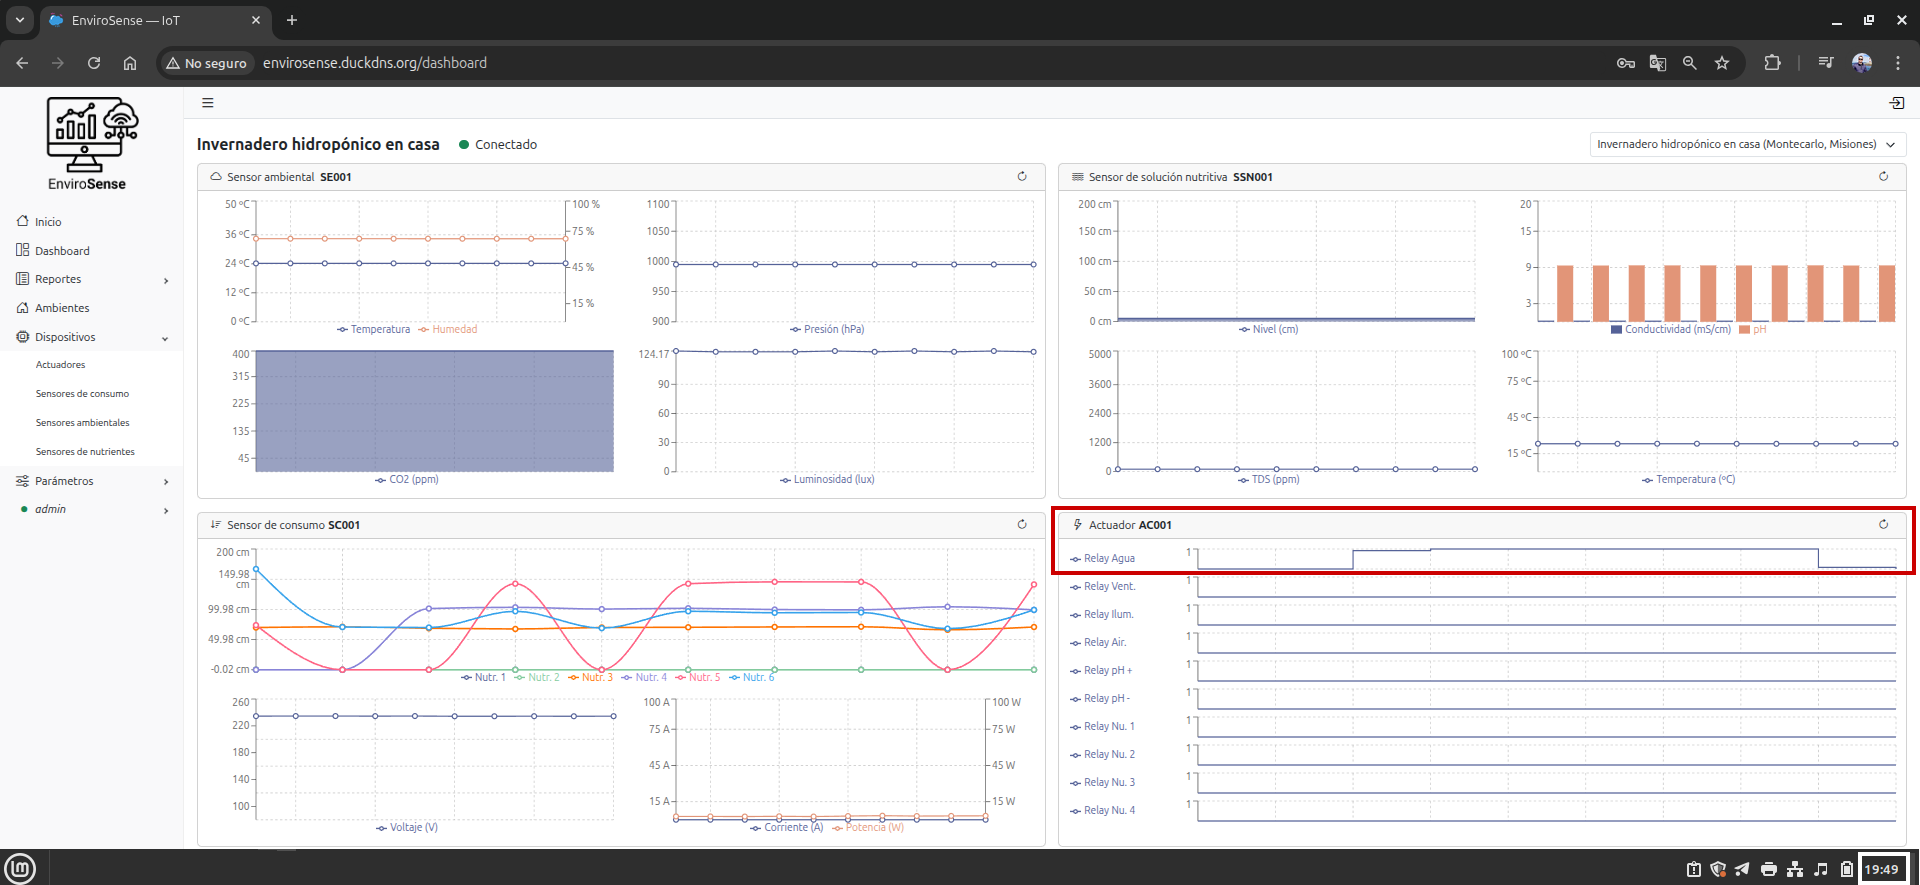
\includegraphics[width=\textwidth]{Images/59_prueba_integral_7.png}
    \caption[Actualización del estado de los relés en el frontend]{Actualización del estado de los relés en el frontend.}
    \label{fig:prueba_integral_7}
\end{figure}
